%%%%%%%%%%%%%%%%%%%%%%%%%%%%%%%%%%%%%%%%%
% Masters/Doctoral Thesis 
% LaTeX Template
% Version 2.5 (27/8/17)
%
% This template was downloaded from:
% http://www.LaTeXTemplates.com
%
% Version 2.x major modifications by:
% Vel (vel@latextemplates.com)
%
% This template is based on a template by:
% Steve Gunn (http://users.ecs.soton.ac.uk/srg/softwaretools/document/templates/)
% Sunil Patel (http://www.sunilpatel.co.uk/thesis-template/)
%
% Template license:
% CC BY-NC-SA 3.0 (http://creativecommons.org/licenses/by-nc-sa/3.0/)
%
%%%%%%%%%%%%%%%%%%%%%%%%%%%%%%%%%%%%%%%%%

%----------------------------------------------------------------------------------------
%	PACKAGES AND OTHER DOCUMENT CONFIGURATIONS
%----------------------------------------------------------------------------------------

\documentclass[
11pt, % The default document font size, options: 10pt, 11pt, 12pt
%oneside, % Two side (alternating margins) for binding by default, uncomment to switch to one side
english, % ngerman for German
singlespacing, % Single line spacing, alternatives: onehalfspacing or doublespacing
%draft, % Uncomment to enable draft mode (no pictures, no links, overfull hboxes indicated)
%nolistspacing, % If the document is onehalfspacing or doublespacing, uncomment this to set spacing in lists to single
%liststotoc, % Uncomment to add the list of figures/tables/etc to the table of contents
%toctotoc, % Uncomment to add the main table of contents to the table of contents
%parskip, % Uncomment to add space between paragraphs
%nohyperref, % Uncomment to not load the hyperref package
headsepline, % Uncomment to get a line under the header
%chapterinoneline, % Uncomment to place the chapter title next to the number on one line
%consistentlayout, % Uncomment to change the layout of the declaration, abstract and acknowledgements pages to match the default layout
]{MastersDoctoralThesis} % The class file specifying the document structure

\usepackage[utf8]{inputenc} % Required for inputting international characters
\usepackage[T1]{fontenc} % Output font encoding for international characters

\usepackage{afterpage}

\usepackage{mathpazo} % Use the Palatino font by default

\usepackage[backend=bibtex,style=authoryear,natbib=true]{biblatex} % Use the bibtex backend with the authoryear citation style (which resembles APA)

\addbibresource{example.bib} % The filename of the bibliography

\usepackage[autostyle=true]{csquotes} % Required to generate language-dependent quotes in the bibliography

%----------------------------------------------------------------------------------------
%	MARGIN SETTINGS
%----------------------------------------------------------------------------------------

\geometry{
	paper=a4paper, % Change to letterpaper for US letter
	inner=2.5cm, % Inner margin
	outer=3.8cm, % Outer margin
	bindingoffset=.5cm, % Binding offset
	top=1.5cm, % Top margin
	bottom=1.5cm, % Bottom margin
	%showframe, % Uncomment to show how the type block is set on the page
}

%----------------------------------------------------------------------------------------
%	THESIS INFORMATION
%----------------------------------------------------------------------------------------

\thesistitle{Application of machine learning techniques to weather forecasting} % Your thesis title, this is used in the title and abstract, print it elsewhere with \ttitle
\supervisor{} % Your supervisor's name, this is used in the title page, print it elsewhere with \supname
\examiner{} % Your examiner's name, this is not currently used anywhere in the template, print it elsewhere with \examname
\degree{Doctor of Philosophy} % Your degree name, this is used in the title page and abstract, print it elsewhere with \degreename
\author{Pablo Rozas Larraondo} % Your name, this is used in the title page and abstract, print it elsewhere with \authorname
\addresses{} % Your address, this is not currently used anywhere in the template, print it elsewhere with \addressname

\subject{Machine Learning} % Your subject area, this is not currently used anywhere in the template, print it elsewhere with \subjectname
\keywords{} % Keywords for your thesis, this is not currently used anywhere in the template, print it elsewhere with \keywordnames
\university{\href{http://www.ehu.es}{University of the Basque Country (UPV/EHU)}} % Your university's name and URL, this is used in the title page and abstract, print it elsewhere with \univname
\department{\href{http://www.sc.ehu.es/ccweb/index.htm}{Computer Science and Artificial Intelligence Department}} % Your department's name and URL, this is used in the title page and abstract, print it elsewhere with \deptname
\group{\href{http://www.sc.ehu.es/ccwbayes/index.html}{Intelligent Systems Group}} % Your research group's name and URL, this is used in the title page, print it elsewhere with \groupname
\faculty{\href{https://www.ehu.eus/en/web/informatika-fakultatea/home}{Computer Science Faculty of San Sebastian}} % Your faculty's name and URL, this is used in the title page and abstract, print it elsewhere with \facname

\AtBeginDocument{
\hypersetup{pdftitle=\ttitle} % Set the PDF's title to your title
\hypersetup{pdfauthor=\authorname} % Set the PDF's author to your name
\hypersetup{pdfkeywords=\keywordnames} % Set the PDF's keywords to your keywords
}

\begin{document}

\frontmatter % Use roman page numbering style (i, ii, iii, iv...) for the pre-content pages

\pagestyle{plain} % Default to the plain heading style until the thesis style is called for the body content

%----------------------------------------------------------------------------------------
%	TITLE PAGE
%----------------------------------------------------------------------------------------

\begin{titlepage}
\begin{center}

\begin{figure}[h]
 \centerline{
\includegraphics[width=10cm]{ehu-upv.png}}\label{logo}
\end{figure}

%\vspace*{.06\textheight}
{\scshape\LARGE \univname\par}\vspace{1.5cm} % University name

\textsc{\Large Doctoral Thesis}\\[0.5cm] % Thesis type

\HRule \\[0.4cm] % Horizontal line
{\huge \bfseries \ttitle\par}\vspace{0.4cm} % Thesis title
\HRule \\[1.5cm] % Horizontal line
 
\begin{minipage}[t]{0.4\textwidth}
\begin{flushleft} \large
\emph{Author:}\\
{\authorname} % Author name - remove the \href bracket to remove the link
\end{flushleft}
\end{minipage}
\begin{minipage}[t]{0.4\textwidth}
\begin{flushright} \large
\emph{Supervisors:} \\
\supname{}Prof. Jos\'e A. Lozano Alonso \\ Prof. I\~naki Inza Cano% Supervisor name - remove the \href bracket to remove the link  
\end{flushright}
\end{minipage}\\[3cm]
 
\vfill

\large \textit{A thesis submitted in fulfillment of the requirements\\ for the degree of \degreename}\\[0.3cm] % University requirement text
\textit{in the}\\[0.4cm]
\groupname\\\deptname\\[2cm] % Research group name and department name
 
\vfill

{\large Donostia - San Sebasti\'an, \today}\\[4cm] % Date
%\includegraphics{Logo} % University/department logo - uncomment to place it
 
\vfill
\end{center}
\end{titlepage}

%----------------------------------------------------------------------------------------
%	DECLARATION PAGE
%----------------------------------------------------------------------------------------

\begin{declaration}
\addchaptertocentry{\authorshipname} % Add the declaration to the table of contents
\noindent I, \authorname, declare that this thesis titled, \enquote{\ttitle} and the work presented in it are my own. I confirm that:

\begin{itemize} 
\item This work was done wholly or mainly while in candidature for a research degree at this University.
\item Where any part of this thesis has previously been submitted for a degree or any other qualification at this University or any other institution, this has been clearly stated.
\item Where I have consulted the published work of others, this is always clearly attributed.
\item Where I have quoted from the work of others, the source is always given. With the exception of such quotations, this thesis is entirely my own work.
\item I have acknowledged all main sources of help.
\item Where the thesis is based on work done by myself jointly with others, I have made clear exactly what was done by others and what I have contributed myself.\\
\end{itemize}
 
\noindent Signed:\\
\rule[0.5em]{25em}{0.5pt} % This prints a line for the signature
 
\noindent Date:\\
\rule[0.5em]{25em}{0.5pt} % This prints a line to write the date
\end{declaration}

\cleardoublepage

%----------------------------------------------------------------------------------------
%	QUOTATION PAGE
%----------------------------------------------------------------------------------------

\vspace*{0.2\textheight}

\noindent\enquote{\itshape Climate is what we expect, weather is what we get.}\bigbreak

\hfill Mark Twain

%----------------------------------------------------------------------------------------
%	ABSTRACT PAGE
%----------------------------------------------------------------------------------------

\begin{abstract}
\addchaptertocentry{\abstractname} % Add the abstract to the table of contents
Weather forecasting is, still today, a human based activity. Although computer simulations play a major role in modelling the state and evolution of the atmosphere, there is a lack of methodologies to automate the interpretation of the information generated by these models. This doctoral thesis explores the use of machine learning methodologies to solve specific problems in meteorology and focuses on the exploration of metodologies to improve the accuracy of numerical weather prediction models using machine learning. The work presented in this manuscript contains two different approaches using machine learning. In the first part, classical methodologies, such as multivariate non-parametric regression and binary trees are explored to perform regression on meteorological data. In this first part, we particularly focus on forecasting wind, where the circular nature of this variable opens interesting challenges for classic machine learning algorithms and techniques. The second part of this thesis, explores the analysis of weather data as a generic structured prediction problem using deep neural networks. Neural networks, such as convolutional and recurrent networks provide a method for capturing the spatial and temporal structure inherent in weather prediction models. This part explores the potential of deep convolutional neural networks in solving difficult problems in meteorology, such as modelling precipitation from basic numerical model fields. The research performed during the completion of this thesis demonstrates that collaboration between the machine learning and meteorology research communities is mutually  beneficial and leads to advances in both disciplines. Weather forecasting models and observational data represent unique examples of large (petabytes), structured and high-quality datasets, that the machine learning community demands for developing the next generation of scalable and capable algorithms. 

\end{abstract}

%----------------------------------------------------------------------------------------
%	ACKNOWLEDGEMENTS
%----------------------------------------------------------------------------------------

\begin{acknowledgements}
\addchaptertocentry{\acknowledgementname} % Add the acknowledgements to the table of contents
There are so many people I would to thank for helping me and supporting me along these years. I will try to keep this list as brief as possible.

\begin{itemize}
  \item To both my PhD supervisors Prof. Jose Antonio Lozano and Prof. Inaki Inza Cano for their guidance and patience.
  \item To the Australian National University and the National Computational Infrastructure for their support in carrying out the last part of this research. 
  \item To my family and friends for being there during these years offering their unconditional love. 
\end{itemize}

\end{acknowledgements}

%----------------------------------------------------------------------------------------
%	LIST OF CONTENTS/FIGURES/TABLES PAGES
%----------------------------------------------------------------------------------------

\tableofcontents % Prints the main table of contents

\listoffigures % Prints the list of figures

%\listoftables % Prints the list of tables

%----------------------------------------------------------------------------------------
%	ABBREVIATIONS
%----------------------------------------------------------------------------------------

%\begin{abbreviations}{ll} % Include a list of abbreviations (a table of two columns)

%\textbf{LAH} & \textbf{L}ist \textbf{A}bbreviations \textbf{H}ere\\
%\textbf{WSF} & \textbf{W}hat (it) \textbf{S}tands \textbf{F}or\\

%\end{abbreviations}

%----------------------------------------------------------------------------------------
%	PHYSICAL CONSTANTS/OTHER DEFINITIONS
%----------------------------------------------------------------------------------------

%\begin{constants}{lr@{${}={}$}l} % The list of physical constants is a three column table

% The \SI{}{} command is provided by the siunitx package, see its documentation for instructions on how to use it

%Speed of Light & $c_{0}$ & \SI{2.99792458e8}{\meter\per\second} (exact)\\
%Constant Name & $Symbol$ & $Constant Value$ with units\\

%\end{constants}

%----------------------------------------------------------------------------------------
%	SYMBOLS
%----------------------------------------------------------------------------------------

%\begin{symbols}{lll} % Include a list of Symbols (a three column table)

%$a$ & distance & \si{\meter} \\
%$P$ & power & \si{\watt} (\si{\joule\per\second}) \\
%Symbol & Name & Unit \\

%\addlinespace % Gap to separate the Roman symbols from the Greek

%$\omega$ & angular frequency & \si{\radian} \\

%\end{symbols}

%----------------------------------------------------------------------------------------
%	DEDICATION
%----------------------------------------------------------------------------------------

\dedicatory{I would like to dedicate this work to Kate, Amaia and Tomas who, one by one, came into my life during this time and made it all possible.} 

%----------------------------------------------------------------------------------------
%	THESIS CONTENT - CHAPTERS
%----------------------------------------------------------------------------------------

\mainmatter % Begin numeric (1,2,3...) page numbering

\pagestyle{thesis} % Return the page headers back to the "thesis" style

% Include the chapters of the thesis as separate files from the Chapters folder
% Uncomment the lines as you write the chapters

% Chapter 1

\chapter{Introduction} % Main chapter title

\label{Chapter1} % For referencing the chapter elsewhere, use \ref{Chapter1} 

%----------------------------------------------------------------------------------------

% Define some commands to keep the formatting separated from the content 
\newcommand{\keyword}[1]{\textbf{#1}}
\newcommand{\tabhead}[1]{\textbf{#1}}
\newcommand{\code}[1]{\texttt{#1}}
\newcommand{\file}[1]{\texttt{\bfseries#1}}
\newcommand{\option}[1]{\texttt{\itshape#1}}

%----------------------------------------------------------------------------------------

\section{Contents and structure}

This doctoral thesis is conceived with the objective of publishing its research outcomes on peered reviewed publications, as a way of measuring its relevance and impact within the meteorological and machine learning communities. At the moment of the defense of this thesis, two manuscripts have been published, another manuscript was presented in a workshop held as part of a well known machine learning conference and a third paper has been submitted to a weather forecasting journal. This document aims to provide the reader with an understanding of the context and research lines pursued by the author during the completion of this work.

\medskip

This first chapter introduces the reader to the field of weather forecasting and its intersection with machine learning. It provides context about the theory behind numerical weather simulations and a historical perspective about the evolution and current state of weather models. Chapter 2 provides an introduction to the main research lines established for this doctoral work  addressing the motivating challenges and main scientific outcomes. Chapter 3 reflects on the overall contributions presenting new avenues and lines of work that we consider promising but did not have the opportunity to explore further. Four appendixes at the end of this thesis contain the original material published by the different journals and conference proceedings. 

%----------------------------------------------------------------------------------------

\section{The origins and evolution of weather forecasting}

Weather forecasting is defined as the application of science and technology to predict the conditions of the atmosphere for a given location and time in the future \citep{vasquez2009weather}. Historically, humans have tried to understand the behavior of the atmosphere by studying the different patterns and relationships between phenomena relating them with future events. For example, it is well known since centuries ago that a sudden descent in the barometric pressure was often followed by precipitation events.

\medskip

In 1922, L. F. Richardson proposed the use of basic fluid mechanics equations to model the movements of the atmosphere. At that time, there was not way to automate calculations, so the author came up with the idea of splitting the surface of the Earth in cells and using persons to solve the differential equations that describe the movements of the atmosphere. According to his estimations, an army of 64,000 human computers would be required to generate an updated forecast for the whole planet \citep{richardson1922weather}. Figure \ref{human_forecasters}, represents the building conceived by Richardson to host his idea of a human "forecasting factory". Unfortunately, due to the proportions of this project, Richardson's idea was never implemented and the availability of a global weather forecast had to wait two more decades. 

\medskip

\begin{figure}[h]
 \centerline{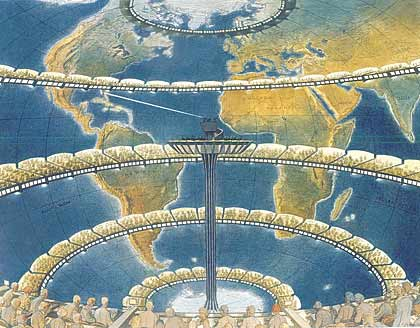
\includegraphics[width=6cm]{human_forecasters.jpg}} \caption{Representation of Richardson's idea of a “forecast factory”, that would employ some sixty-four thousand human computers sitting in tiers around the circumference of a giant globe solving the equations to forecast the weather. (Source: \url{http://cabinetmagazine.org/issues/27/foer.php}).}\label{human_forecasters}
\end{figure}

At the end of World War II, when electronic computers and atmospheric radio sounding data became available, the United States led an ambitious project to implement the first automated forecasting system. In 1950 meteorologists Jule Charney, Agnar Fjörtoff, and mathematician John von Neumann published a paper named "Numerical Integration of the Barotropic Vorticity Equation" \citep{charney1950numerical}, which establishes the basis for computer weather models setting the foundations of Numerical Weather Prediction (NWP) as we know it today. This work resulted in the implementation of the first weather forecast by electronic computer. The model was implemented and run operationally on the ENIAC computer, at the University of Pennsylvania. Due to the capacity limitations of this computer, it took 24 hours of processing time to generate a 24 hour forecast, which limited its applications, as it could not effectively predict the future.

\medskip

Since the 1950s computers have been used to simulate the state and evolution of the atmosphere using Numerical Weather Prediction models \citep{kimura2002numerical}. These models use a set of nonlinear differential equations to approximate the state and evolution of the atmosphere, which are known as the primitive equations. These primitive equations define the conservation of mass, momentum and thermal energy. The primitive equations are solved by NWP models using finite difference, or spectral methods, for the three dimensions of the space and time. NWP models initialise these equations using observed data, to create a snapshot of the state of the atmosphere. This process is known as "analysis" \citep{courtier1994strategy}. To integrate the different parameters simulated through these equations, the Earth is divided in a discrete grid representing the evolution of the different regions of the atmosphere through time. Figure \ref{N80} represents the distribution of grid points in a regular Gaussian grid.

\medskip

\begin{figure}[h]
 \centerline{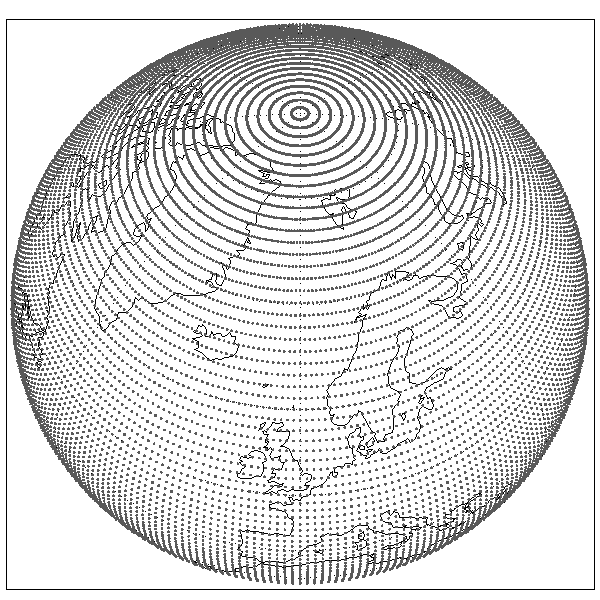
\includegraphics[width=9cm]{N80_regular.png}} \caption{Example of an F80 regular Gaussian grid used by some NWP to represent the Earth's atmosphere (Source: \url{https://www.ecmwf.int}).}\label{N80}
\end{figure}

NWP models are therefore built using mathematical equations that describe the dynamical physical processes in the atmosphere. To simulate the future state of the atmosphere the same set of equations are solved iteratively using the output of the previous step. This process is repeated until the solution reaches the desired forecast time. However, errors in the simulated variables accumulate through time and the accuracy of the computed forecast deteriorates at each step. Using too coarse grid cells or long integration time steps are the main causes for NWP errors. The contribution of the small scale or sub-grid processes, which are not explicitly resolved by the physical equations in the model, becomes significant. Increasing the spatial and temporal resolution of NWP partially solves this problem but at the cost of significantly increasing the computational requirements of the model.

\medskip

One of the main constraints limiting NWP is the resolution of the grid used to resolve the equations, which is usually in the order or kilometers. This resolution is usually smaller than the natural scale of some important atmospheric processes. Processes such as convention, radiative transfer or cloud formation happen at smaller scales than models can explicitly resolve. For these small-scale or complex processes, NWP models use simplified or approximated processes called parameterisations \citep{milton1996impact,delage1997parameterising}. 

\medskip

Parameterisations are one of the most complicated components of NWPs. Parameterising small-scale processes correctly becomes crucial when forecasting events more than 48 hours in advance, when the effect of these processes usually becomes significant. Parameterisations are usually built using simplified models to approximate atmospheric processes. These models are often defined by discretising a process into different categories, where different linear models are applied in each case. Parameterisations for different processes are sometimes closely related and have to be specified in conjunction resulting in non-trivial interactions and dependencies. Figure \ref{CFS} contains a representation of the output of the National Oceans and Atmosphere Administration (NOAA) Climate Forecast System (CFS) representing  the global atmospheric precipitable water, which is a parameterised variable. 

\medskip

\begin{figure}[h]
 \centerline{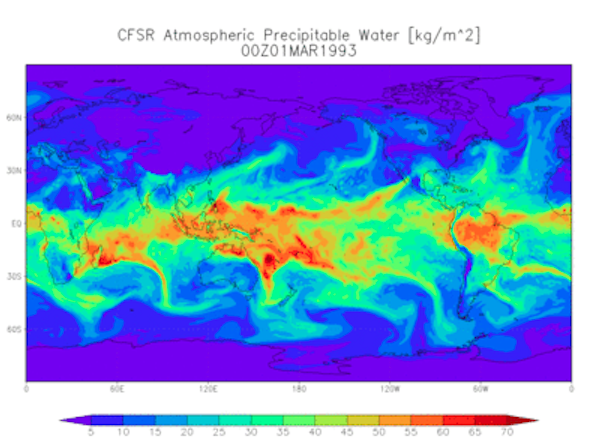
\includegraphics[width=9cm]{CFS.png}} \caption{NOAA CFS output for the global atmospheric precipitable water on March 15, 1993 for a 12-hour accumulation period (Source: \url{https://www.ncdc.noaa.gov}).}\label{CFS}
\end{figure}

Another consequence of the NWP grid resolution is the limitation in accounting for the effect of topography. Global NWP models use a coarse representation of the shape and features of the surface of the Earth, averaging coastlines and mountain heights over the extent of the corresponding grid cell, which is normally in the order of 10 to 100 kilometers. As a consequence, they are unable to represent important local effects that happen at a sub-grid scale.

\medskip

Another major constraint that physical NWP models suffer is the difficulty to represent the chaotic nature of the atmosphere \citep{lorenz1982atmospheric}. The mathematical equations governing the dynamics of the atmospheric flows are nonlinear and they represent non-stable hydrodynamical and thermodynamical processes. Small differences in the initial state can amplify as the system evolves resulting in significantly different scenarios. NWP models are initialised in the analysis phase using observational data which has an intrinsic uncertainty associated with them. This uncertainty can be propagated through time resulting in a variability in the results. The instability of the atmosphere defines an upper and lower bound on the predictability of instantaneous weather patterns.

\medskip

At the beginning of the 1990's, the meteorological community proposed ensemble forecasting as a methodology to measure the predictability of the atmosphere using NWP \citep{molteni1996ecmwf}. Instead of making a single high resolution simulation, ensemble forecasts run a set of forecasts with slightly different initial conditions. This set of forecasts provide an indication of the range of possible future states of the atmosphere and possible scenarios. Figure \ref{ensemble} represents the evolution of the temperature variable represented as a transformation in the shape of its probability distribution through time. The different members normally aggregate around different values which correspond to the most likely scenarios for a given physical parameter.

\medskip

\begin{figure}[h]
 \centerline{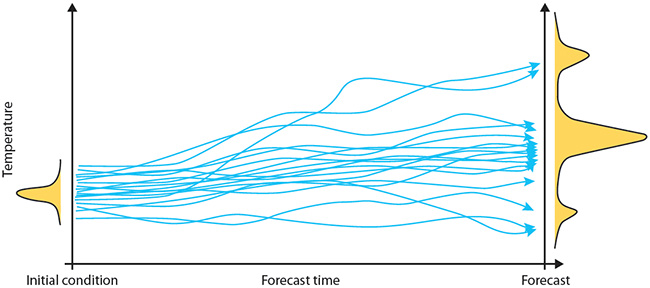
\includegraphics[width=10cm]{ensemble-forecasting.jpg}} \caption{An ensemble of forecasts produces a range of possible scenarios given an initial probability distribution of a forecasted parameter. The different ensemble members provide an indication of the possible resulting scenarios based on a probability distribution. (Source: \url{https://www.ecmwf.int}).}\label{ensemble}
\end{figure}

\medskip

As we have seen, the representation of non-linear subgrid processes and the quantification and propagation of uncertainty are central to the process of weather forecasting. The former is closely related to the scale of the equations used to represent the atmospheric physical processes and the latter to the precision of the sensors and the confidence we have in their measurements.

%----------------------------------------------------------------------------------------


\section{Numerical weather prediction}

As introduced in the previous section, computers have been used since the 1950's to simulate the state and evolution of the atmosphere. Ever since this time, capacity of the computers has doubled every 18 months following Moore's Law and similarly the resolution of the weather models. Although the physical equations and methodologies for resolving them have remained fundamentally the same as in the first weather models, the spatial and temporal resolution as well as the frequency of the runs of the models has been constantly increased up until nowadays. In terms of the accuracy -- skill in the weather forecasting literature -- of the forecasts, NWP performance has improved by two days per decade, as shown in Figure \ref{model_improvement}. This means that the accuracy of a 4-day forecast today is as good as it was 10 years ago for a 2-days forecast.

\medskip

\begin{figure}[h]
 \centerline{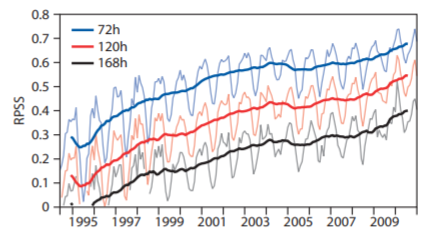
\includegraphics[width=10cm]{model_skill.png}} \caption{The performance of the EPS has improved steadily since it became operational in the mid-1990s, as shown by this skill measure for forecasts of the 850 hPa temperature over the northern hemisphere at days 3, 5 and 7. Comparing the skill measure at the three lead times demonstrates that on average the performance has improved by two days per decade. The level of skill reached by a 3-day forecast around 1998/99 (skill measure = 0.5) is reached in 2008-2009 by a 5-day forecast. In other words, today a 5-day forecast is as good as a 3-day forecast 10 years ago. The skill measure used here is the Ranked Probability Skill Score (RPSS), which is 1 for a perfect forecast and 0 for a forecast no better than climatology. (Source: \url{https://www.ecmwf.int}).}\label{model_improvement}
\end{figure}

The field of NWP verification has been extensively studied in the field of weather forecasting \citep{ahijevych2009application}. The need for methods that can measure the accuracy and quality of the information produced is fundamental to identify weaknesses in the simulation of the atmospheric processes. The two baselines that are often used to measure the quality of the forecasts are persistence in short range (0-2 days) forecasts and climatology in mid- (2-5 days) to long-range (5+ days) forecasts. Persistence is the assumption that the meteorological conditions are going to stay the same. In this context a NWP model needs to be better at forecasting the weather than a simple model that keeps the variables constant in time. The climatology baseline, on the other hand, assumes that the weather is going to behave as the averaged historical records for that particular area.

\medskip

One of the main limitations of NWP models has been the lack of observations over large regions of the world, which limited the initialisation of the initial state of models, which is called "analysis". For a long time, the conditions over the Pacific ocean or the southern hemisphere were vastly unknown due to a lack of ground station and atmospheric sounding data. This limitation has been greatly improved since the introduction of satellites and remote sensors. Since the 1990s satellite data has become available and the assimilation of these data by NWP models has resulted in an significant improvement in the quality of their forecasts. This is a trend that is expected to continue, as new satellites equiped with new and more capable sensors become available. For example, in August 2018, a joint initiative of the European Union and the European Space Agency (ESA) has launched Aeolus, the first satellite able to monitor the Earth's winds. This satellite alone is expected to significantly increase the accuracy of NWP models by providing valuable information of the winds with a global coverage.

\medskip

The synoptic scale in meteorology (also known as large scale or cyclonic scale) is a horizontal length scale of the order of 1000 kilometers or more. NWP models have been able to simulate the presence and evolution of the synoptic atmospheric systems since the beginning. This comprises phenomenons such as mid-latitude depressions, fronts and most high and low-pressure areas seen on weather maps. As the size of the grid cells used to simulate the weather has been reduced, models have been able to simulate atmospheric processes happening at lower scales. Current models are able to explicitly solve the processes that occur at the mesoscale level, which comprises phenomena that manifest at scales ranging 5 to 100 km, such as sea breezes, squall lines or medium to large-sized convective cells. Current global weather models operate at a resolution that ranges 25 to 100 km which allows for partially accounting for some of these mesoscale systems. There are important phenomena such as convection, turbulence, radiative processes or raindrop coalescence that occur at the micro-scale level, which comprises scales smaller than 5 km. NWP models cannot explicitly solve the physical equations ruling these processes.

\medskip

The physical variables simulated by NWP can be separated in two main types, depending on the nature of the equations used to simulate them. Basic parameters are the ones explicitly computed by NWP solving the physical equations. Examples of these are atmospheric pressure, wind, temperature or humidity. Derived parameters are the ones that are not explicitly solved by NWP but are derived from basic parameters using parameterisations. Precipitation, convection, heat radiative processes or turbulence are examples of derived parameters. 

\medskip

Due to the relatively coarse resolution of NWP models, there are considerations to be made relatively to the representativeness of its variables and their interpretation at specific grid cells. Figure \ref{model_resolution} compares the topography of Europe using two different resolutions. As it can be seen, the level of detail varies significantly between both representations and important details in mountainous and coastal areas cannot be represented using coarse representations. This implies that NWP models cannot account for the impact that topography has on weather variables at scales lower than its grid cell's size. 

\medskip

\begin{figure}[h]
 \centerline{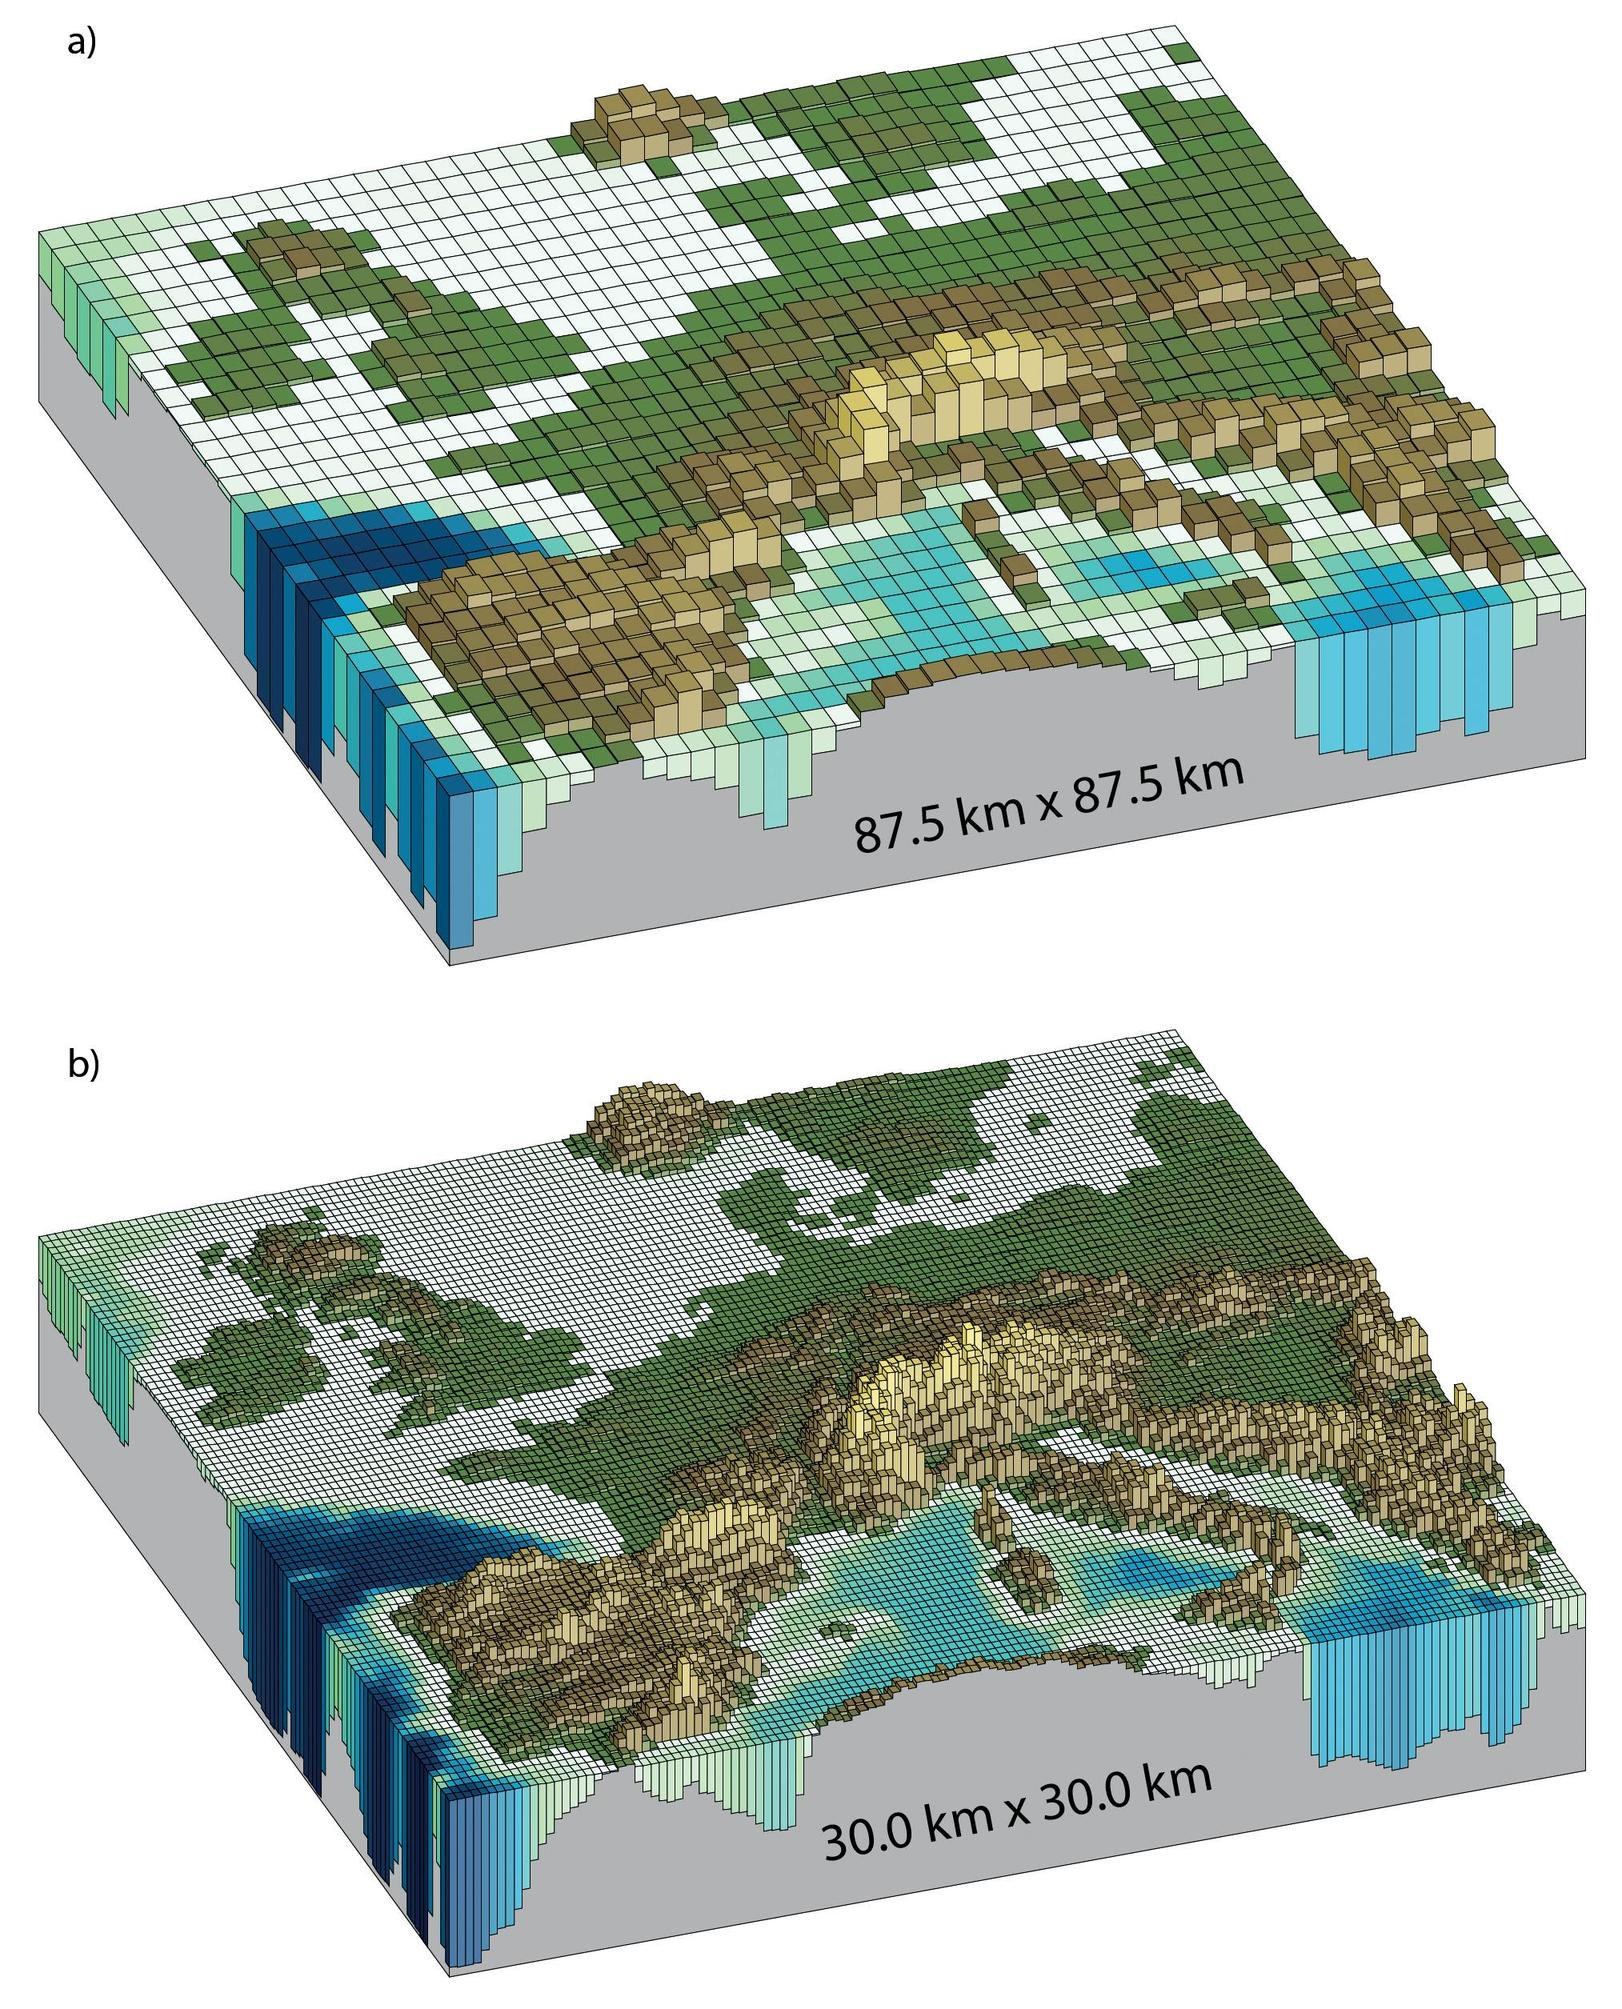
\includegraphics[width=10cm]{nwp_resolution.jpg}} \caption{Comparison between the horizontal resolutions used in global models today [30 km] (a) and the equivalent models 10 years ago [87.5 km] (b). (Source: \url{http://www.climatechange2013.org}).}\label{model_resolution}
\end{figure}

A common problem in NWP data interpretation is to infer high-resolution information from low-resolution variables. This process is called "downscaling" in disciplines such as meteorology, climatology or remote sensing. This process can be based on dynamical or statistical approaches such as splines, kriging or nesting into higher resolution models \citep{peng2017review}. Machine learning based methods lie in the category of statistical methods, and they can be used to improve the output of NWP learning and extracting patterns of the relationship between the model's historical output and their corresponding observed values.

\medskip

NWP models are complex systems which are usually developed by large organisations during decades. Their development requires a high degree of specialisation on different areas and entire teams of highly skilled scientists are dedicated to different components of the model. Models are often designed using modules which can be run with a certain independence from the rest of the system. However, the atmosphere is a complex system in which most of its variables are interlinked defining dependencies and feedback processes between them. NWP are highly optimised to run on High Performance Computing (HPC) facilities using Fortran and C and libraries such as OpenMP \citep{dagum1998openmp} and MPI \citep{gropp1999using} to distribute the computation between large compute clusters and accelerate the generation of its output. 

%----------------------------------------------------------------------------------------

\section{The sources of weather data}

So far, we have focused our attention on NWP, as this is currently the only tool available that is able to "forecast" the evolution and future estate of the different physical parameters describing the atmosphere. However, NWP output is not the only source of information when studying the atmosphere. Sensors, under many forms and characteristics, provide accurate values of the observed conditions in a region of the atmosphere. Examples of sensors used in weather forecasting are: ground stations, atmospheric sounding balloons, weather radars or satellites. Each of these types of sensors has different characteristics in terms of the spatial and temporal resolution and the extent that they can cover.

\medskip

Observational data sets are crucial in the process of weather forecasting as they provide a live stream of information describing the current state of the atmosphere. Forecasters use these data operationally to validate the NWP output and to correct for possible errors or local effects. 

\medskip

Specially relevant to this thesis work are METARs, which are weather observation reports generated in most of the airports in the world. These reports are used to plan air traffic control in airports and are one of the highest quality observed data sources available. The following code represents a METAR report for the airport of Donostia, Spain. The code starts with the International Civil Aviation Organization code of the airport, date of the report, wind conditions, visibility, cloud coverage, temperature and finishes with the pressure conditions.

\texttt{LESO 071119Z 31013KT 280V340 3000 RA FEW018 SCT033 BKN040 14/12 Q1020}

\medskip

NWP models also combine all the different sources of observed data to establish the initial conditions of the model. This process, which is known as "analysis phase", is a complex process in which all the different sources of information, together with the previous output of the NWP model, need to be combined in a consistent manner. Figure \ref{gos_wmo} represents some of the most important sensor data that are used to initialise NWP models.

\medskip

There are mainly two techniques used to perform the analysis of NWP models: Ensemble Kalman Filter (EKF) \citep{burgers1998analysis} and 4-Dimensional Variational assimilation (4D-Var) \citep{courtier1994strategy}. These techniques basically integrate the different variables across the space and time minimising a cost function that measure the difference between the observed values and the ones in the NWP.

\medskip

\begin{figure}[h]
	\centerline{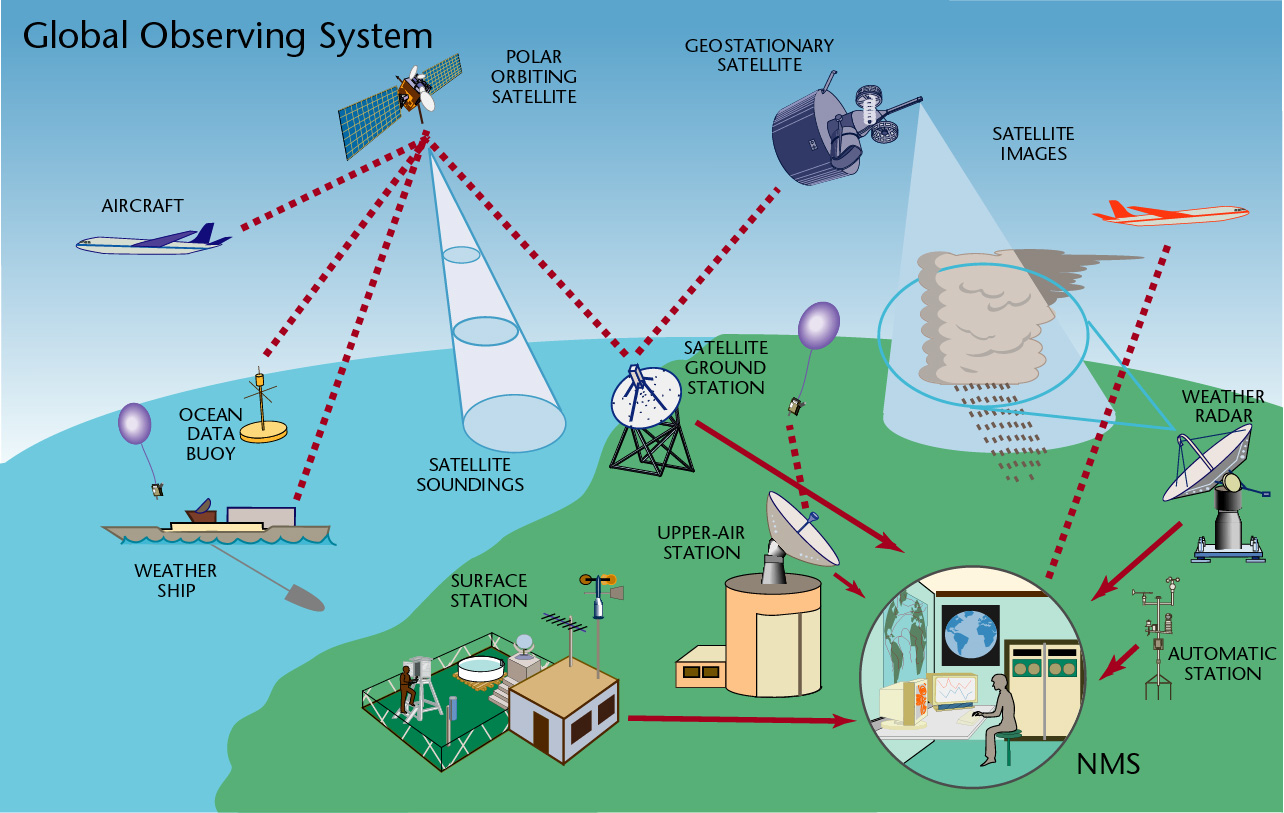
\includegraphics[width=12cm]{GOS-fullsize.jpg}} \caption{ The Global Observing System (GOS) consists of a network of synoptic surface-based observations made at over 11000 land stations, by about 7000 ships and 750 drifting buoys at sea and around 900 upper-air stations, together with reports from aircraft and remotely sensed data from geostationary and polar orbiting satellites. (Source: \url{http://www.wmo.int/pages/prog/www/OSY/GOS.html}).}\label{gos_wmo}
\end{figure}

Historical observational data sets are kept in the records of the different weather organisations for performing climatological and research studies. A special kind of NWP models, called climatic or re-analysis models, simulate the state of the atmosphere in the past instead of in the future. These models are produced as a way of having a consistent dataset that represents the weather of the past. These data sets are mainly used for performing research studies about the evolution of the atmosphere during the last years or centuries, depending on the temporal extent and resolution of the model. Examples of these models are ERA-Interim \citep{dee2011era} and CMIP5 \citep{taylor2012overview}.  

\medskip

Weather agencies around the world provide access to weather forecasts, severe weather warnings, observations, flood information and climate information to society. The amount of information generated by these centres is very large and its storage and management requires high capacity infrastructure to support it. The volume of some of these collections is in the order of Petabytes of information. For example, ERA5, one of the latest reanalysis data sets, has generated nearly 6 Petabytes of data. Although these data sets have been historically maintained in tape storage systems, there is an increasing demand to consume these data in real-time, which requires high-performance storage file systems \citep{evans2015nci}.

\medskip

Weather data is mostly represented using multidimensional numerical arrays. There are specific file formats, such as NetCDF-4 \citep{rew2006netcdf} or HDF5 \citep{folk2011overview}, which are optimised to provide fast access to the whole data or subsets of it implementing advanced compression techniques to reduce the size of the files. These formats also implement metadata standards to ensure the compatibility and interoperatibility of the files between organisations.

\medskip

The high volumes of data generated at simulating the atmosphere and an increasing interest in these data by sectors such as agriculture, air and maritime transport or renewable energies, pose a challenge on how to make these data available. Currently, large investments are dedicated to infrastructure to facilitate the access to weather data by the public. Multiple national and international efforts, such as the European Copernicus program \citep{copernicus}, are currently focused on designing and implementing new systems capable of processing and extracting value out of weather and climate data.

\medskip

More generally, the ready availability of large datasets about the Earth has awaken the interest on combining different sources into new studies and analysis, coining the \textit{data fusion} term \citep{wald1999some}. One of the biggest challenges when combining data from different sources is the heterogeneity of the data. Data coming from different NWP models or satellites is represented using different combinations of grids, units, projections, spatial and temporal resolutions and file formats. The process of data fusion is normally preceded by a laborious and error prone process to homogenise the data into a common representation. This process is commonly known as \textit{data wrangling} \citep{goldston2008big} and, unfortunately, is a common activity in weather sciences. For example, downscaling of NWP output constitutes an active field of research in meteorology which usually requires the combination of low resolution gridded NWP data with other higher resolution sources such as local weather stations or Earth Observation (EO) \citep{giebel2011state,renzullo2016improved}.

\medskip

During the last decade there has been an increasing interest coming from private companies into weather and Earth observation datasets. Weather datasets have been recently made available by large cloud computing companies, such as Amazon or Google. Also, these companies are investing on systems to access and process these large datasets using their infrastructure \citep{gorelick2017google,earthaws}. This offers a new avenue for the use of these data, which has been historically dependent on the support of large national agencies and computational infrastructures.

\medskip

These initiatives are popularising and democratising the access of the general public to weather data sets. However, the Cloud presents quite different architecture when compared to traditional High Performance Computing (HPC) centres. Systems, models and file formats have been developed during the last half century based on mature and stable technologies, such as POSIX file systems and the x86 CPU architecture. There is nowadays an unprecedented opportunity to redesign the systems that will bring weather data into new applications and ubiquitous uses in society.

\medskip

This transition making weather data more accessible is happening at the same time to the development of new machine learning and large scale analytics algorithms. Due to the size of these datasets, computers have replaced humans as the main consumers of data. This trend is expected to continue with the release of new algorithms capable of analysing weather data and produce on-demand added value products \citep{cloudai,awsml}.

%----------------------------------------------------------------------------------------

\section{Machine learning}

The term "machine learning" dates back to the middle of the last century. In 1959, computer scientist Arthur Samuel defined machine learning as "the ability to learn without being explicitly programmed." \citep{samuel1959some}. Machine learning can also be seen as a particular way to solve a more generic task expressed with the concept of "artificial intelligence", which involves machines being able to think and reason in a similar way to what humans do. The concept of "artificial intelligence" predates the one of "machine learning" by a few years. In 1950, Alan Turing published a groundbreaking paper with titled "Computing machinery and intelligence" \citep{machinery1950computing}, in which the question of whether machines can think was formally raised. In 1956, John McCarthy, computer scientist at Stanford University, used this term to express the idea that machines can simulate any form of human learning.

\medskip

There are different ways of defining and representing the intersection between "artificial intelligence" and "machine learning". Depending on the author and scientific field, these terms are often found in conjunction with others, such as "computational statistics" or "data science". In the context of this thesis, we use the term "machine learning" to refer to the field of computer science that uses statistical techniques to give computer programs the ability to "learn" from data. This section introduces some of the main areas and algorithms in machine learning, with special emphasis in those that have been applied in this doctoral work to solve specific weather forecasting problems.

\medskip

One of the main challenges in machine learning is to design generic algorithms that can find meaningful representations in the data. In practice, input data is usually adapted through a series of transformations to suit the requirements of a specific algorithm. For example, designing an algorithm that is able to extract the time from images of wall clocks is a non-trivial problem. If the same wall clock images are processed resulting in a new dataset that contains the angles of the clock hands for each image, the complexity of the problem is reduced significantly. This problem is called representation or feature learning \citep{bengio2013representation}.

\bigskip
\bigskip

\fbox{%
    \parbox{0.9\textwidth}{%
        \textit{Representation of features becomes a central topic of research in the first half of this thesis. Weather data and specifically wind data, is naturally represented as vectors defining the speed and directional components. The directional component is represented by a circular variable that, as opposed to linear variables, is not bounded. If represented in radians, this means that a circular variable with the value of 0 represents the same point in the variable space as 2$\pi$. Most of the machine learning algorithms are not designed to work with circular variables and fail to represent them correctly. In our work, we explore methods to improve the representation of circular variables through use cases that contain wind direction, time and calendar date variables.}
    }%
}

\bigskip
\bigskip

From the point of view of the nature of the problem that machine learning algorithms try to solve, we can differentiate two main classes of learning problems: supervised and unsupervised. Supervised learning \citep{russell2016artificial} consists on extracting relationships or patterns in the data, given a dataset which includes an output tag or value for each input element. Supervised algorithms learn the relationships between the input and output and, after being trained, can infer or predict the output of new input data. On the other hand, unsupervised learning problems \citep{hastie2009unsupervised} require the algorithms to extract the inherent structure in the data without using explicitly-provided labels or output values. The distinction between supervised and unsupervised problems allows the classification of machine learning algorithms in two categories. However, there is an spectrum of interesting problems that lay in between both. Semi-supervised learning \citep{chapelle2009semi}, falls between unsupervised learning and supervised learning exploring the use of unlabeled data mixed with a small amount of labeled data for training. More generally, weakly supervised learning \citep{hernandez2016weak} deals with scenarios in which data sets present missing or inaccurate labels or target values. 

\medskip

Regression algorithms fit in the category of supervised learning and their purpose is to estimate the value of a continuous output variable using a set of input variables. In mathematics, a linear system can be solved when we know a number of equations that is equal to the number of variables in the system. Linear regression presents the problem of having a data set normally containing a much larger number of points than variables in the data, which is referred as an overdetermined system. Regression finds a solution to such system by minimising the overall error.

\medskip

The most basic algorithm to perform regression is linear regression \citep{neter1989applied}, which uses a linear function to relate the input or independent variables with an output or dependant variable. The following equation represents the linear relationship between one output element of the dataset and a set of \textit{n} input variables:

\[ y = \beta_1 x_{1} + \beta_2 x_{2} + ... + \beta_n x_{n} + \epsilon \]

There are many approaches to solve linear regression models, which are all based on minimising the error, represented by the $\epsilon$ value in the equation, across the whole dataset.  Least-squared methods are normally used to perform linear regression. Most implementations require a matrix inversion which makes the computational cost of these methods grow with the dimension of the data. An alternative approach is to use iterative methods, such as gradient descent, to make the model converge minimising the error value. 

\medskip

Linear regression models, although simple and effective in many situations, do not provide good representations when the data presents non-linear relationships. Non-linear regression methods allow training models that are able to represent non-linear relationships between the input variables. There are many methods to define non-linear methods such as Taylor or sinusoidal series, or by segmenting the space and using a series of linear regression models, also called piece-wise regression.

\medskip

Non-linear regression models are more capable of representing relationships in the data than linear models. However, the larger capacity of non-linear regression models can lead to data representations with excessive detail. If the model learns to reproduce, with high precision, the relationships in the training dataset, sometimes is an undesirable effect as it can fail to generalise new data points, unseen during the training phase. This problem is known as overfitting \citep{hawkins2004problem} and its effect is represented in Figure \ref{overfitting}. In this figure, we can see a non-linear regression model accurately representing all the points in a data set, as opposed to a linear model that approximates its values. In some cases, the linear model can provide a better representation of the problem than the non-linear version, and we'll say that the non-linear model is overfitting the data. Sometimes, overfitting can be easily solved by adding more data to the model. In other situations, avoiding overfitting requires a careful consideration about the model design and its parameters.

\medskip

\begin{figure}[h]
 \centerline{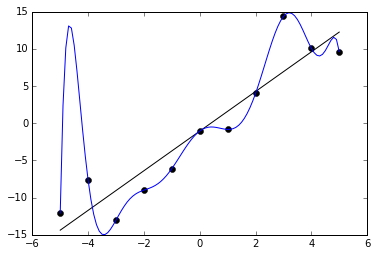
\includegraphics[width=10cm]{overfitting.png}} \caption{Comparison of a non-linear regression model (blue) and a linear model (black) representing a 2-dimensional data set. Source: Creative Commons by M. Giles}\label{overfitting}
\end{figure}

Another alternative for performing non-linear regression are the, so called, non-parametric regression methods. In non-parametric regression, there is not a single model that represents the whole data set. The model is constructed ad hoc for each individual case, according to the information derived from the data. Non-parametric regression models search the dataset looking for the elements that are "closer" to the input value. Therefore, they often require larger data sets than the equivalent parametric methods. 

\medskip

Kernel regression is a particular method of non-parametric regression. Kernel regression uses mathematical window functions, called kernels, to weight the contribution of input data points. This method estimates a continuous dependent variable from a limited set of data points, which the kernel selects by weighting the contribution of each data point, giving higher weights to nearby locations. Figure \ref{kernel_shapes} shows seven different kernel functions which apply different weighting patterns to the data.

\medskip

\begin{figure}[h]
 \centerline{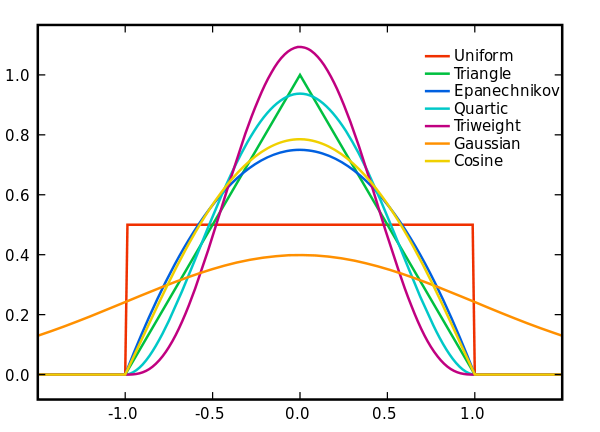
\includegraphics[width=10cm]{kernel_shapes.png}} \caption{Comparison of the shape of seven common window functions used in kernel regression. Source: Creative Commons by Brian Amberg}\label{kernel_shapes}
\end{figure}

\bigskip
\bigskip

\fbox{%
    \parbox{0.9\textwidth}{%
        \textit{Kernel regression is the method used in the first contribution of this doctoral thesis. It was used to resolve the local effects of local topography and improve the NWP forecasted wind speed values at airports. Cyclic kernels can be used to filter historical wind observations by their directional component. The resulting models provide a dynamic regression model that can account for the effects of surrounding physical features of an area, such as mountains or coast lines.}
    }%
}

\bigskip
\bigskip

There is an area within regression that is specifically focused on analysing time-series data. The objective of these methods is to predict future values based on the short- and long-term trends and patterns in the data. This problem has been traditionally approached by the statistical community by applying auto-regressive methods, such as Auto-Regressive Moving Average (ARMA) or Auto-Regressive Integrated Moving Average (ARIMA), to predict the future state or transitions of temporal and sequential variables \citep{stram1986temporal,zhang2003time}. \textit{(Although weather forecasting can be regarded as a highly dimensional time-series problem, these methodologies have a limited application at predicting the weather. NWP achieves significantly better results by explicitly simulating the physical equations of the atmosphere typically with hourly resolutions.)}

\medskip

We have covered some methodologies used to perform statistical regression on data based on least-squared like methods. However, there are other well known ways of building models from data that represent continuous variables. Decision trees, for example, provide a tool to model relationships in the data by partitioning the dataset space into independent regions. The algorithm of Classification and Regression Trees (CART), proposed by Leo Breiman in 1984 \citep{breiman1984classification}, is based on the use of binary decision trees to generate classification and regression models. 

\medskip

Regression trees perform a recursive partitioning of a dataset based on a metric that maximises the homogeneity in the resulting children nodes, such as the variance. At each node of a binary regression tree, one variable is selected to perform a partition by selecting one value; typically data points with values larger than the splitting value end up in one child node and the smaller ones are assigned to the other child node. This partitioning process is performed until a stop criteria is met, usually based on the number of data points or a minimum variance value per node. When a node is no longer partitioned, it is called a leaf.

\medskip

Regression trees provide an easy and intuitive way to model data. They are fast to train, scale well with large data sets and are easy to interpret and understand by looking at the decisions made at each node of the tree. These factors have contributed to their popularity, and nowadays regression tree applications can be found at nearly any field of science. There are many versions or possibilities to build regression trees and, since their invention, many authors have presented alternative methods to build trees, presented new metrics or proposed ways of pruning trees to better represent the data \citep{quinlan2014c4,freund1999alternating}. 

\medskip

Regression tree algorithms perform significantly better when trained in groups or ensembles \citep{breiman1996bagging}. Bagging, also known as bootstrap aggregation, is an ensemble tree method used to reduce the variance of individual decision trees. The different tree members of the ensemble are created using sub-data sets by randomly selecting data points, with replacement, from the training data. The average of all the individual predictions from the ensemble trees provides a more robust predictor than any of the individual regression trees. Ensemble methodologies have also become very popular and there is a wide range of algorithms available such as boosting or random forest \citep{dietterich2000experimental,breiman2001random}.

\bigskip
\bigskip

\fbox{%
    \parbox{0.9 \textwidth}{%
        \textit{The second contribution in this doctoral thesis proposes a new methodology to build regression trees that can incorporate circular variables. Based on a previous pioneering work that introduces circular trees, we build up and extend this concept with an alternative method that generates better partitions of the circular space. The methodology restricts the options to partition a circular variable by only allowing splits that generate contiguous regions, in a similar way to how linear variables are handled in classic regression trees.}
    }%
}

\bigskip
\bigskip

Alternatively to the covered methods, there are other kind of algorithms for performing regression that are often more capable of representing high-dimensional data sets and non-linearities in the data. Two very popular examples are Support Vector Machines (SVM) \citep{hearst1998support} and multilayer feed-forward Artificial Neural Networks (ANN) \citep{hornik1989multilayer}. Both these methodologies use a series of "basis functions" to define hyperplanes and represent the data. Non-linearities in the data can be represented by using the "kernel trick" \citep{mika1999fisher} in SVM and activation functions in ANN. Although there are similarities between SVM and multilayer feed-forward ANN, the former is non-parametric and has variable size whereas the latter is parametric and has fixed size defined by the number and dimensions of its layers. Later in this section we come back to ANNs in the context of image analysis and deep learning.

\medskip

The field of machine learning that studies structured and high-dimensional data sets is commonly known as "structured prediction" \citep{taskar2005learning}. Structured prediction, studies methodologies to deal with regular and large output spaces. Datasets representing temporal or spatial dimensions are typically found in this field \citep{gupta2010estimating,tran2012max}. Spatial data analysis has received special attention in engineering, for its applications in robotic vision and autonomous vehicles defining the field of computer vision.

\medskip

Computer vision has been historically focused on the development of methods based on engineered features, such as SIFT \citep{lowe2004distinctive} and HOG \citep{dalal2005histograms}, which have been the standard approach for applying machine learning to images and other high-dimensional regular gridded data. Another approach has been feature construction \citep{guyon2006introduction}, which does require to manually define the characteristics of the different features in an algorithm. Feature construction makes use of simple but effective algorithms which can achieve satisfactory results for certain tasks \citep{blum1997selection}. However, in the last decade, new methodologies based on the use of convolutional neural networks, have demonstrated to be more generic providing substantial advantages over previous methodologies. 

\medskip

Deep Learning \citep{lecun2015deep} methods have recently achieved unprecedented results in different supervised classification and regression tasks, using different kinds of high dimensional data sets, such as images or audio. These methods use large artificial neural networks composed of tens or in some cases hundreds of layers. Recent research has presented networks that are capable of surpassing human-level performance at different complex tasks such as image classification \citep{krizhevsky2012imagenet} or semantic description \citep{karpathy2015deep}. Deep learning networks for image analysis are normally based on Convolutional Neural Networks (CNN) \citep{krizhevsky2012imagenet}, which have been proven to be very effective at capturing intrinsic features represented at different scales of an image. CNNs learn several layers of convolutional kernels, which are able to establish local connections between nearby pixels in the image. Each layer in the network performs a sampling operation immediately after the convolution, reducing the dimensions of the image. Kernels in one layer cover larger areas than in the previous layer. The network is able to progressively aggregate the spatial features of images, creating high level representations.

\medskip

Convolutional encoder-decoder networks are a type of CNN that provide state-of-the-art results at tasks such as image segmentation \citep{badrinarayanan2017segnet}, image denoising \citep{mao2016image} or image-to-image regression \citep{isola2017image}. These networks are based on autoencoders \citep{hinton2006reducing}, which use CNNs to learn reduced but accurate representations of images, generalising its use to find relationships between different images. Convolutions in the encoder half of the network perform a feature selection process by reducing the dimensionality of the data. The decoder part enlarges the feature space mapping it to the output space. Encoder-decoder networks offer an effective method for learning the relationship between high dimensional input and output spaces, such as the ones defined by images or video.

\medskip

Convolutional encoder-decoder networks have recently opened an active and promising field of research in areas such as medicine \citep{greenspan2016guest}, astronomy \citep{shallue2018identifying} or high-energy physics \citep{baldi2014searching}. In the field of weather and climate sciences there is also an incipient interest in the introduction of convolutional networks to perform analysis and interpretation of NWP weather and climate data sets.

\bigskip
\bigskip

\fbox{%
    \parbox{0.9 \textwidth}{%
        \textit{Our third contribution applies convolutional encoder-decoder networks, originally designed to perform image segmentation tasks, to model the relationships between atmospheric variables. Convolutional encoder-decoder networks can learn to extract the 3-dimensional spatial structure represented by pressure fields from NWP, and predict precipitation. This application becomes specially relevant in the field of weather forecasting, as precipitation is a parameter that is not explicitly resolved by NWP and it is modeled or parameterised instead. This method provides therefore a viable alternative to generate parameterisations in NWP models.}
    }%
}

\bigskip
\bigskip


\medskip










%----------------------------------------------------------------------------------------

\section{Weather forecasting: The machine learning approach}

Before the existence of NWP models, humans used a simple technique to forecast the weather based on the observed data collected over the years for a specific region, which is known as climatology. Rough estimations about long-range trends and cumulative values of variables, such as temperature or precipitation, can be inferred by applying basic statistics to observed weather events over long-enough periods of time.

\medskip

At the beginning of the 20\textsuperscript{th} century, with the advent of the technology to accurately measure the atmosphere and to communicate these values across geographically distant places, weather maps became available. These maps initially started representing the position and shape of the low and high pressure systems and allowed the development of the weather forecasting methodologies, which predicted the movement and effects of these pressure system in the atmosphere. The application of statistical models to weather forecasting was proposed as early as in the 1950's \citep{malone1955application}. At the same time that the first NWP models were developed, Malone presented the argument that "statistics must eventually play some role" in the simulation of the atmosphere. The author demonstrated a methodology, using multiple linear regression, to forecast the sea-level pressure field. Figure \ref{regression_meteo} shows this first attempt of using regression methods to predict the evolution of the surface temperature at Indianapolis (USA). This model uses the atmospheric circulation pressure field in the previous 24 hours as input to forecast the next 24 hours.

\medskip

\begin{figure}[h]
 \centerline{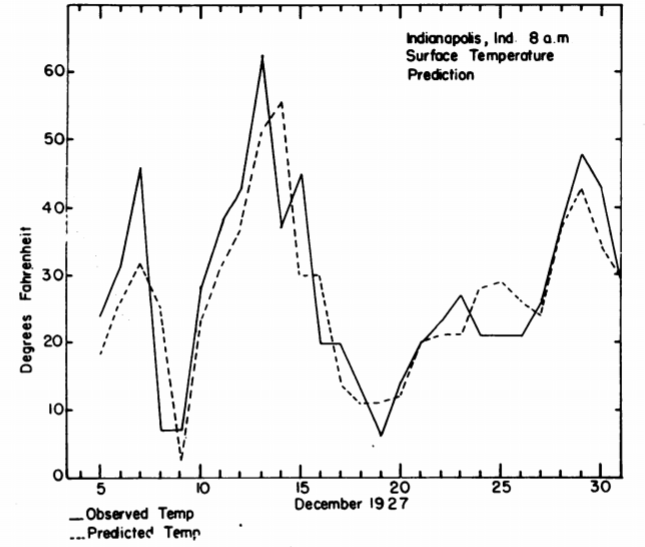
\includegraphics[width=10cm]{regression_meteo.png}} \caption{This figure represents a comparison between a 24-hour prediction of daily mean temperature and the observed temperature values at Indianapolis (USA). Source \citep{malone1955application}}\label{regression_meteo}
\end{figure}

Although pure statistical based methodologies have not yet been able to replace NWP simulations in forecasting the weather, statistics have played a major role in complementing and enhancing the output of NWP. It is well known that forecasts from NWP models have certain defects that can be removed by statistically post-processing their output \citep{wilks1995forecast}. 

\medskip

Statistical models, used for post-processing NWP output, have evolved within three general frameworks: "Perfect Prog", Model Output Statistics (MOS), and Reanalysis \citep{marzban2006mos}. "Perfect Prog" models \citep{vislocky1989use} use regression to represent the relationship between the initial state of NWP (analysis) variables, such as temperature or precipitation, and observations of those same parameters \citep{klein1959objective}. The trained models are then used to correct NWP forecasted fields, such as temperature or precipitation, rectifying deficiencies in the NWP forecast. "perfect Prog" assumes that the accuracy of the forecast does not depend on the size of the forecasting window. In contrast, MOS fits a linear regression model between NWP output at a certain forecast time with observations at that time \citep{glahn1972use}. Because MOS fits the NWP output directly, it can correct for biases and systematic errors in a model. When NWP model configurations are updated, MOS must be retrained after a sufficient number of new model forecasts are collected. "Perfect Prog" models are generally less accurate than an optimised MOS model, but they are less sensitive to model configuration changes and tend to be more robust over time. In the development of all the variations on MOS and "Perfect Prog", a limitation is the amount of data available for training the regression models \citep{mcgovern2017using}. The use of reanalysis data to train allows developing post-processing models similar to "Perfect Prog" and MOS without the limitation in the amount of observed data \citep{kalnay2003atmospheric}.

\medskip

Linear regression models have been used in weather forecasting within a broader context than removing bias from NWP simulated fields. For example, regression methods have been proposed to downscale extreme precipitation events from NWP data \citep{friederichs2007statistical}. Similarly \citep{rozas2014method} propose a form of parametric regression based on the use of kernels to resolve the local effects of winds non resolved by NWP. We can find other applications of regression to forecast the probability of severe weather \citep{kitzmiller1995wsr} or the maximum hail size and its probability \citep{billet1997use}. In cases where the output is not a continuous variable but a binary outcome or a set of categories, logistic regression can be used to forecast the occurrence of certain events such as convective processes \citep{mecikalski2015probabilistic} or the selection of NWP ensemble members \citep{messner2014heteroscedastic}.

\medskip

One of the main limitations of linear regression based models is that not all the relationships between the different atmospheric processes and its variables can be modeled using linear functions. Also, least-squared based methods used to solve linear regression, such as matrix inversion, do not scale well when a dataset presents a large number of input variables. To overcome these limitations different methods have been proposed in the literature, such as multilevel regression used to model climatic variability for non-linear processes \citep{kravtsov2005multilevel} or quadratic regression for the generation of ensemble members \citep{hodyss2013square}. In the case of having a large number of input variables or when these variables are closely related, the training process of regression models can be difficult. For example, ridge regression based techniques have been proposed as a method to select variables in multi-model scenarios \citep{delsole2013scale} where different models forecast the same variables with different levels of accuracy. Least Absolute Shrinkage and Selection Operator (LASSO) is another technique, similar to ridge regression, that has been applied to weather forecasting problems for NWP downscaling \citep{hofer2017evaluating} or long-range seasonal forecasting \citep{delsole2017statistical}. Also, Principal Component Analysis (PCA) methods have been proposed to parameterise sub-grid scale processes in the atmosphere \citep{godfrey2010empirical}.

\medskip

Regression and classification tree based methods are a popular approach to model non-linear atmospheric processes. Before tree methods became popular in the 1980's, decision trees were introduced to provide diagnosis of upper-level humidity levels in the atmosphere \citep{chisholm1968diagnosis}. Trees can be easily scaled to train models using large data sets and with high number of input variables. The easy interpretability of the trained models has also contributed to the popularisation of these methods in weather forecasting. Decision tree based methods have proven to be a powerful tool in a wide variety of weather applications, such as the detection and diagnosis of thunderstorm turbulence \citep{williams2008remote}, extreme precipitation events \citep{herman2018money}, or to represent the circular nature of wind \citep{larraondo2018system}. Figure \ref{decision_tree} represents a decision tree for predicting hail precipitation \citep{mcgovern2017using}, which clearly communicates a method that human forecasters can follow to forecast hail.

\medskip

\begin{figure}[h]
 \centerline{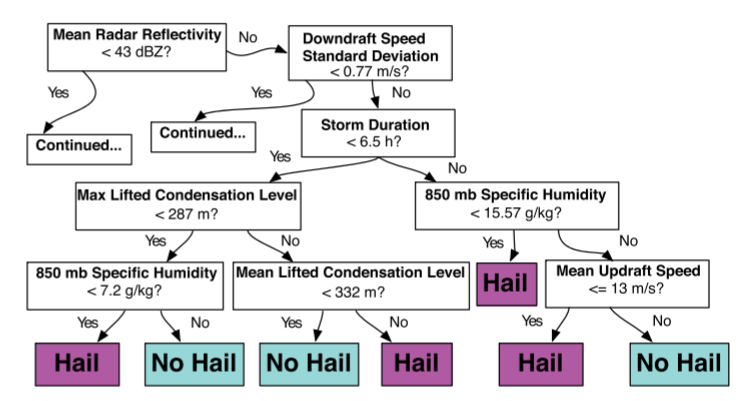
\includegraphics[width=10cm]{decision_tree.png}} \caption{Example of a decision tree used to forecast the event of hail based on thresholds for different observed and NWP parameters. Source \citep{mcgovern2017using}}\label{decision_tree}
\end{figure}

Tree based methods are able to represent non-linearities in the data through a piece-wise approximation, by recursively splitting the input space. Artificial Neural Networks (ANN), Support Vector Machines (SVM) or Support Vector Regression (SVR) provide a generic, more powerful alternative to modeling non-linear processes. Both ANN and SVM/SVR models are flexible and powerful, but produce models that are often difficult to interpret in terms of underlying physical concepts that the model has identified. This characteristic has limited the application of such models to weather forecasting problems, in domains where scientists require an understanding of the assumptions made by the model due to the need of coupling with other models or the need to account for inter-dependencies between variables. ANNs suffer a similar problem where the resulting models are difficult to interpret through the weights and nonlinear activation functions. ANNs have been used in a wide variety of meteorology applications since the late 1980s \citep{key1989classification}, with applications such as cloud classification \citep{bankert1994cloud}, tornado prediction and detection \citep{marzban2006mos}, cloud height and visibility \citep{marzban2007ceiling}, precipitation classification \citep{anagnostou2004convective} or bias correction for precipitation and temperature forecasts \citep{moghim2017bias}. ANNs have recently expanded into deep learning methods, whose applications in the field of weather forecasting are covered at the end of this section. SVM and SVR based methods have also been extensively used in weather applications such as to detect and predict tornadoes \citep{adrianto2009support} or for forecasting precipitation \citep{wei2012wavelet,liu2015wavelet} 

\medskip

Another common task in weather forecasting is the identification of groups of models or regions that present similar meteorological situations, for performing classification or create clusters of probable scenarios in ensemble forecasting models. Clustering algorithms, such as k-means, allow analysing weather information in an unsupervised manner. Clustering algorithms have been proposed in the literature to solve tasks such as precipitation map segmentation \citep{baldwin2005automated}, precipitation distribution patterns using hierarchical clustering \citep{ramos2001hierarchical}, El Ni\~{n}o pattern identification  \citep{johnson2013enso}, or to predict typhoon trajectories \citep{camargo2007cluster}.

\medskip

In spite of the optimism expressed by Malone in the early 1950's \citep{malone1955application} through his early results demonstrating the use of pure statistical methods to forecast the weather, the reality is that the application of machine learning methods has come as a complement of NWP rather than as an alternative to it. The power of the physical equations to simulate the evolution of the atmosphere within the spatial and temporal dimensions has not yet been matched by other methods. We have seen in this section how different machine learning methodologies have been applied to solve a broad range of problems in the field of weather forecasting. Depending on the task to be solved and the nature of the underlying data, we can identify the following categories of problems where machine learning approaches have been applied:

\medskip

\begin{itemize}
  \item Correction of NWP systematic error: This category comprises the cases where NWP output data is post-processed to remove biases, increase the output resolution or include local topographic effects using observed data \citep{aznarte2017dynamic,buehner2010intercomparison}.
  \item Predictability assessment: Due to the chaotic nature of the atmosphere, weather forecasts have an intrinsic uncertainty value associated, which limits its value. Machine learning methods have been used to assess the uncertainty and associated confidence scores of ensemble forecasting \citep{wilks2002smoothing,foley2012current,mallet2009ozone}.
  \item Extreme detection: This category groups classification problems in which the outcome is the prediction or detection of a rare event. Examples of these applications are found in methods that predict phenomena such as hail, wind gusts or cyclones \citep{mcgovern2017using,williams2008remote,herman2018money}.
  \item NWP parameterisations: NWP models generate multiple variables using approximate models or parameterisations to describe processess which cannot be simulated through explicit physical equations. Although these parameterisations have been historically based on empirical models, the use of machine learning is starting to grow. There are examples of machine learning methods applied to model processes, such as radiative transfer, convective and boundary-layer or turbulence \citep{szturc2007parameterisation,o2018using,gentine2018could}.
\end{itemize}

\medskip

Most examples of machine learning applications found in the literature require a drastic simplification or reduction in the dimensionality of the data. NWP and remote sensing systems generate large amounts of information, which is represented using high dimensional numerical arrays. These multi-dimensional arrays or tensors represent the state and evolution of the atmosphere through space and time using a large number of variables. Due to the volume of data, machine learning applications in weather forecasting, often limit the input space to individual grid points in space or time. Generalising these models usually requires the use of parametric approaches or training multiple versions of the same models for different points in time and space. This approach requires large processing power and is difficult to scale. Also, implementations of traditional machine learning algorithms, such as linear regression, tree based methods or artificial neural networks are designed to work on reduced input spaces and their complexity quickly becomes unmanageable as the number of input variables grows \citep{raible1999statistical,bowler2006steps}. Training models on highly dimensional spaces has remained a challenge in the field of machine learning \citep{fan2013mining} and has prevented the development of substantial alternatives to NWP for simulating the weather. 

\medskip

There has been a strong focus in the machine learning community to explore new methodologies that can be applied to large volumes of data or high dimensionalities. In particular deep learning methods \citep{lecun2015deep} have demonstrated state-of-the-art results using large data sets \citep{deng2009imagenet,openimages}. The application of these methodologies has also been recently explored in the field of weather forecasting with unprecedented results \citep{xingjian2015convolutional,liu2016application,rasp2018deep}.

\medskip

Deep neural network models have demonstrated to effectively and efficiently extract complex patterns from large structured data sets. Specifically, Convolutional Neural Networks (CNNs) provide a methodology to extract spatial information from image data sets. Similarly, Recurrent Neural Networks (RNNs), developed in the field of natural language processing, have found many applications in a broad range of data sets containing the temporal dimension. The combination of both models was first proposed in the context of precipitation now-casting \citep{xingjian2015convolutional} using radar data. Convolutional Long-Short Term Memory (LSTM) networks, a form of RNN, has been popularised afterwards in other domains with structured spatio-temporal datasets. 

\medskip

Figure \ref{deep_clasif} shows the results of a deep learning model trained using a large collection of NWP pressure fields to detect jet-stream flows. This model was trained on a large cluster of compute nodes at the Lawrence Berkeley Supercomputing centre in the USA demonstrating the scalability and capacity of CNNs to extract complex spatial patterns in the data.

\medskip

\begin{figure}[h]
 \centerline{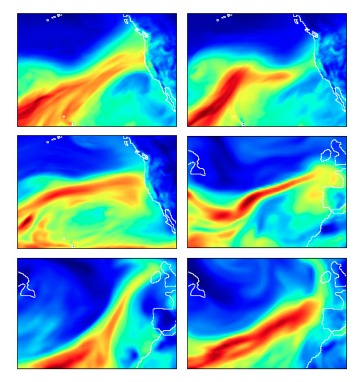
\includegraphics[width=10cm]{deep_classif.png}} \caption{Sample images of atmospheric rivers (jet-streams) correctly classified and extracted from a multi-Terabyte NWP dataset by a deep CNN model. Source \citep{liu2016application}}\label{deep_clasif}
\end{figure}

Also, in the field of deep learning there is a great potential in applying convolutional encoder-decoder networks to learn parameterisations from basic NWP fields (article about precipitation parameterisation submitted to the Monthly Weather Review as part of this doctorate work). Generative models, such as Variational Auto-Encoders (VAE) \citep{kingma2013vae} or adversarial models \citep{goodfellow2014gan} are being explored as ways to simulate variability and understand the stability of specific meteorological situations. This approach can generate variations from a basic meteorological situation similarly to the way ensemble methods operate but using a single model. Although there are not yet publications demonstrating the potential of these methods, several works exploring this idea have been presented in conferences lately.

\medskip

Even if new methodologies demonstrate to be able of learning the physics underneath NWP models, it is hard to imagine that they will substitute NWP, at least in the short- mid-term. Basic fields in NWP, such as pressure or winds are accurately modelled using physical models, which are solved using highly-optimised numerical methods. The code and compilers running these models have been continuously improved during the last 60 years. Machine learning models would still need some time to achieve similar levels of efficiency in running simulations at comparable resolutions than NWP.

\medskip

Regarding the trend in the volume of data generated by NWP models and observation systems during the past decades, we can foresee that the size and complexity of the data sets is going to continue growing at an exponential rate. Interpreting and analysing such volumes of data will require methodologies that are able to extract patterns from large and complex data sets, making an efficient use of the available computational and storage resources. 

\medskip

Assuming the existence of a system capable enough to analyse the whole collection of historical observations of the atmosphere extracting the patterns and spatio-temporal relationships between the variables, such system would be able to replace NWP entirely. In this scenario, there would be no need to understand the physical equations that rule the atmosphere, as algorithms would be able to extract models that simulate it. Figure \ref{nwp_vs_ml}, represents the different approaches taken by NWP and machine learning into the weather forecasting problem.

\medskip

\begin{figure}[h]
 \centerline{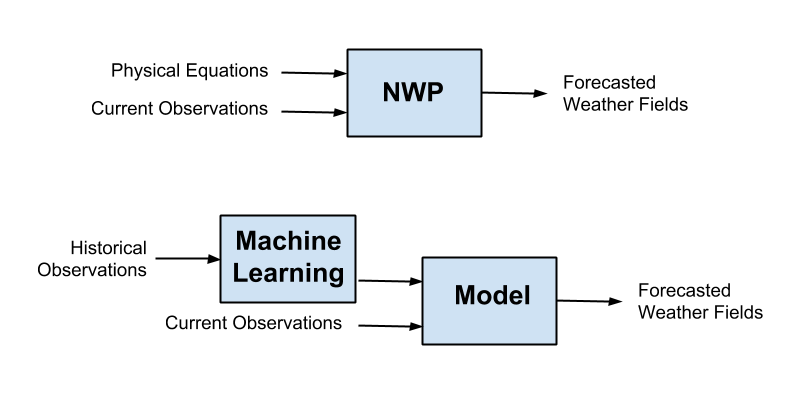
\includegraphics[width=12cm]{nwp_vs_ml.png}} \caption{Comparison of the traditional NWP and machine learning approaches to weather forecasting.}\label{nwp_vs_ml}
\end{figure}

\medskip

NWP and observed data collections from surface and remote sensing sources provide a unique resource for the exploration of structured weather prediction problems. Experts working on different domains of weather and climate modeling agree that we will see a proliferation of automated statistical methods to help interpreting weather information in the near future \citep{jones2017ml}. First, as a complement to NWP, machine learning based methods will help us to have a better understanding of complex processes occurring in the atmosphere and will most likely extend into more generic models, as the efficiency and capacity of the algorithms improves and more computational power becomes available.

\medskip



\ExplSyntaxOn
\NewDocumentCommand{\blankpages}{m}
 {
  \clearpage
  \prg_replicate:nn { #1 } { \mbox{}\thispagestyle{plain}\clearpage }
 }
\ExplSyntaxOff

% Chapter 2

\chapter{Line of research and contributions} % Main chapter title

\label{Chapter2} % For referencing the chapter elsewhere, use \ref{Chapter1} 

\section{Improved wind forecasting using kernel regression for circular variables}

\subsection{Introduction}
The first part of this work is focused on exploring how classic non-linear regression methodologies can be used to improve the output of numerical weather models. Multivariate linear regression is a classic method for modelling the relationship between a scalar output variable and one or more input variables. This method serves in many cases as the baseline method when comparing new approaches to do regression, so we decided to start our research by exploring the most fundamental techniques.

The challenge in this case is to perform regression on the NWP wind speed variable using observed data. Wind is a weather phenomenon that is highly dependent on topography. Wind is normally represented using a vector representation where the wind speed is the module of the vector and wind direction corresponds to its angle. Weather models simplify the simulation of wind by decomposing this vector into its cartesian components. The problem with this approach is that performing operations such as regression is not straight forward because of the relationship and dependence between both components.

For this study, we use the GFS NWP model and Aviation Routine Weather Reports (METARs) from three airports in northern Spain, Vitoria-Gasteiz, Bilbao and San Sebastian-Donostia. The GFS model represents data using a regular grid which covers the whole world, with a spatial resolution of approximately 50 km and a temporal resolution of 3 hours. This model is operated by the National Oceanographic and Atmospheric Administration (NOAA) maintains and the global dataset for the latest 15 years is publicly available to the public. METARS are high quality meteorological reports drafted in most of the civil airports in the world. These reports are made available every 30 minutes and describe variables such as the wind, temperature, visibility and cloud coverage at the airport's runway. METARS are encoded as text messages and distributed worldwide so flight control groups and pilots can plan take off and landing procedures.

For each of the three airports we selected the NWP grid points closest to the observation points, creating a temporal series that contains both the modeled and observed values for different weather parameters. We compare different linear and non-linear regression methodologies using different combinations of NWP variables in the input and using the observed wind speed as the output variable.

The reason for choosing wind speed as the output is because this variable is highly affected by the local topography surrounding the airports. Airports are normally located in open spaces with constant and wind patterns. These three airports in northern Spain are placed in a mountainous region near the Atlantic coast and have very specific wind regimes which are highly affected by the local topography. The resolution of the NWP model used in this study is in the order of 75 km, which means that these three airports are modeled in contiguous grid cells. The work is focused on studying the potential of observed wind speed data to correct the NWP values for specific locations.

\subsection{Research contribution}

Non-parametric regression is a category of regression analysis in which the predictor does not take a predetermined form but is built each time from the data. Non-parametric regression requires larger sample sizes than regression based on parametric models because the data must supply the model structure as well as the model estimates. This work demonstrates a technique using non-parametric regression for improving wind speed prediction by clustering wind speed data around specific directional components. This regression is performed dynamically, selecting historical data with similar characteristics. The level of similarity and the relative weights for each element in the regression is controlled using different shapes of kernels.

\begin{figure}[h]
 \centerline{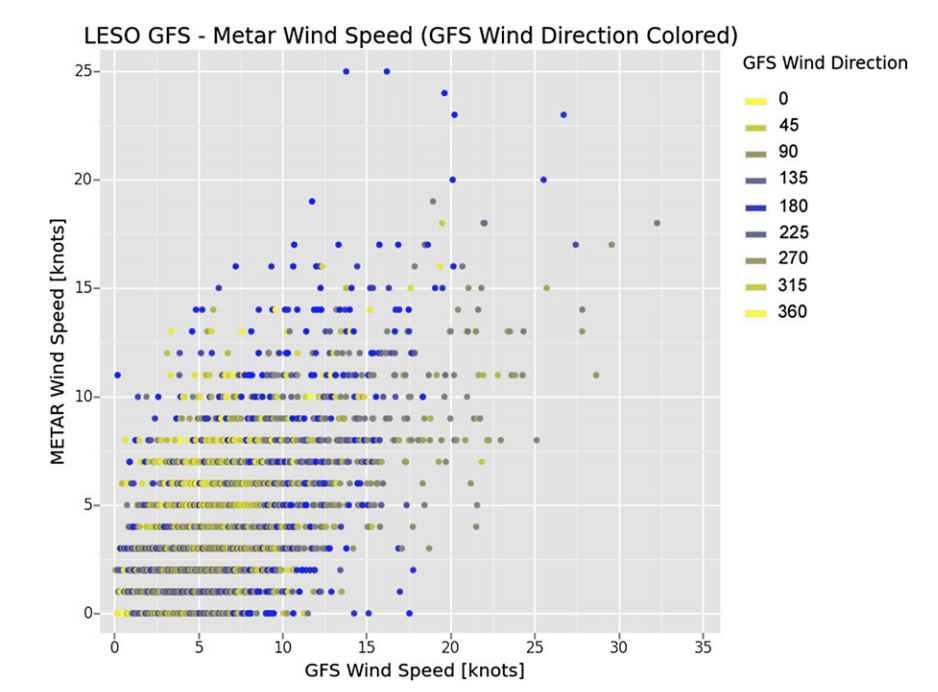
\includegraphics[width=10cm]{paper1.png}}\caption{Relationship between GFS and METAR wind speed values from San Sebastian. GFS wind direction is represented using a color scale, with colors around yellow showing northerly winds and colors around blue representing southerly winds.}\label{paper1}
\end{figure}

For example, Figure \ref{paper1} contains a representation of the correlation between the wind values generated by the NWP and the observed wind in one of the studied airports. Using the wind direction value, we can dynamically assign a weight to each element intervening in the regression.

This work introduces the concept of cyclic kernel which provides a way of clustering elements using a circular variable. We demonstrate how circular kernels can  successfully assimilate
directional data into a regression model. This concept can also extend and improve other circular or temporal variables and can be used to extract seasonal or daily patterns from data.

\subsection{Publication: A Method for Wind Speed Forecasting in Airports Based on Nonparametric Regression}

This work was published in the "Weather and Forecasting" journal, which is a scientific publication from the American Meteorological Society. This publication covers articles on weather forecasting and analysis techniques, forecast verification studies, and case studies useful to forecasters. It was first submitted to the journal in March 2014 and was finally published in December 2014 after a major revision process that required work on improving the statistical method used to validate the methodology.

\blankpages{10}

%----------------------------------------------------------------------------------------

\section{Circular regression trees}

\subsection{Introduction}

Most of the current regression machine learning algorithms are focused on modelling the relationships between linear variables. Circular variables have a different nature to linear variables, so traditional methodologies are not able to represent their content thoroughly, leading to suboptimal results in most cases.

Continuing with the study of methodologies for modelling circular variables, we decided to focus on regression trees for this new research study. Regression trees and tree based ensemble methods, such as bagging or Random Forest, are a versatile, computationally efficient and accurate method for performing regression. Building upon the pioneering concept of circular regression tree \citep{lund2002tree}, we decided to explore alternative and more efficient methods for introducing circular variables in regression trees.

Traditionally, circular variables have been used in regression trees using two approaches. The first one ignores the circular nature of a variable treating it as linear variable. The problem with this approach is that 0 and 360 degrees are represented at each end of the variable range, when in reality they are the same value. The second approach is to decompose a circular variable into its Cartesian components and use them as separate variables in a tree. Both of these approaches introduce constrains and limit the performance of regression trees. With the first approach, trees cannot perform splits that cross the origin, and in the second case splits performed on the Cartesian components independently lead to an excessive and unnatural partition of the space defined by circular variables having a negative impact in the accuracy of the resulting models. 

For this work we use a similar dataset to the one introduced in the previous section about non-linear kernel regession. We choose to forecast the observed speed of the wind at 5 different locations in Europe. Data from airport METARS of Berlin Tegel, London Heathrow, Barcelona El Prat, Paris Charles de Gaulle and Milano Malpensa are used to train the different tree models and to analyse the results. Similarly to the previous work we extract the time series data from the GFS model for the closest grid cells to each of these airports. The tree models are trained using three-hourly data for the years 2011, 2012 and 2013, providing approximately 8760 samples per airport.


\subsection{Research contribution}
The key idea behind circular trees is that circular variables can be naturally integrated in regression trees by considering splits that cross the origin [0-360] point in the search space. The original implementation of circular trees perform splits on non-contiguous regions of the variable space leading to excessive fragmentation of the dataset. The improvement proposed in our work restricts the search space to contiguous regions of the variable space leading to an improvement in compute performance and accuracy of the results, as shown in Figure \ref{paper2}.

In this work we introduce a new methodology that restricts the search space of each partition in a tree generating contiguous partitions. This constraint added to the initial idea of circular regression trees in Lund's work \citep{lund2002tree} has the implication of generating more simple partitions which improve the accuracy of the tree model and is more efficient to train. Although the search space for optimal splits at each node of the tree is more limited than the original version, which allows non-contiguous splits, the overall error of the tree results to be lower as the depth of the tree increases. In this work we found that even if non-contiguous splits provide good results at the top part of a tree, these partitions tend to degenerate as the partition process evolves resulting in trees with poor performance.

\begin{figure}[h]
 \centerline{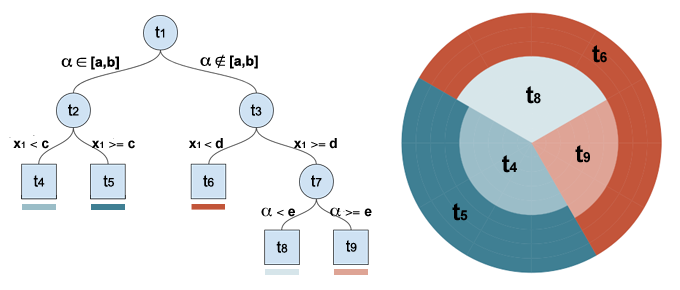
\includegraphics[width=10cm]{paper2.png}}\caption{Example of the proposed circular regression tree and a representation of how the space is divided in contiguous regions.}\label{paper2}
\end{figure}

The software developed in this work is presented in the form of a self-contained Python library. This library implements a general version of regression tree which can be used with both linear and circular variables in the input and output. Also, there is an option to perform non-contiguous partitions, as in the original proposal by Lund and contiguous as in the metodology that we propose.  The library also offers a command line interface that allows users to train and test different regression tree models and download datasets for any airport in the world. These tools have been designed so users can create their own forecasts experimenting and exploring the differences between models, input variables and airports. The scripts and libraries are written in a simple way so users can read the code to understand what the program is doing and also modify or extend its functionalities. AeroCirTree comes with a GNU GPLv3 licence so anyone can use, modify and share this program for any purpose.

\subsection{Publication: A system for airport weather forecasting based on circular regression trees}

In March 2017 it was finally submitted to the "Environmental Modelling \& Software", a peer-reviewed scientific journal which publishes work involving modelling and software within the Environmental science domain. The work was published in February 2018, after a major revision process that required extra work to demonstrate the benefit of our circular methodology to other linear trees alternatives.

\blankpages{10}

%----------------------------------------------------------------------------------------

\section{Convolutional neural networks for image regression}

\subsection{Introduction}
During the time of working on the circular regression tree, deep learning techniques where presented to the research community demonstrating unprecedented results in many different domains. Although, as far as we knew, there were not applications in the meteorological domain in the literature we decided to learn and apply these techniques to weather forecasting problems. Convolutional neural networks, used mainly on image classification tasks, seemed a good candidate to model NWP gridded data.

Up until this point in our research, we extracted data from the closest NWP grid point to the desired observed dataset resulting in a time series. Convolutional Neural Networks (CNN) offer the possibility of treating a whole image as the input to a model and the neural network can learn to detect the regions of the image that are most correlated with the output. This is a major change on how we were doing research compared to our two previous works. CNNs do not require to know the location of the individual grid pointsas an input, they can treat the whole weather grids (images) as their only input avoiding the need of extracting temporal series beforehand.

Convolutional neural networks are mainly used to perform classification and extraction of the spatial information in images, building from fine grained details into higher level structures. In this work we explored the use of CNNs to classify the event of precipitation (rain/dry) at different cities in Europe. 

CNN require large datasets to be trained. For this work we used a different dataset called ERA-Interim \cite{dee2011era} which contains data since the year 1979, with a temporal resolution of 3 hours. This dataset is publicly available from the European Centre for Medium-Range Weather Forecasts (ECMWF). This dataset is generated using a numerical weather model which simulates the state of the atmosphere for the whole planet, with a spatial resolution of approximately 80 km.  The output is presented in the form of regular numerical grids and there is a large number of physical parameters available, representing variables such as temperature, wind speed and relative vorticity.

For determining the event of rain at the different locations we use Aviation Routine Weather Reports (METARs) similarly to our previous works. We consider 5 main airports located in different cities across Europe and a period of 5 years (2012-2017). The airports are: Helsinki-Vanta, Amsterdam-Schiphol, Dublin, Rome-Fiumicino and Vienna.

We extract an extended area over Europe from ERA-Interim, creating a 3 hourly series of images composed by 3 bands, corresponding to the geopotential height \textbf{z} at the 1000, 700 and 500 pressure levels of the atmosphere. This parameter represents the height in the atmosphere at which a certain pressure value is reached. These levels correspond typically to 100, 3000 and 5500 metres above the mean sea level respectively.

\subsection{Research contribution}

In this work we experimented adding the temporal dimension to the CNN network. The temporal dimension is added to these networks by adding a fourth axis to the convolutional kernels (latitude, longitude, height, time). Using the collection of geopotential fields as input and the precipitation conditions for the different locations as output, the CNN networks are able to find the relationships between them. Although the location of the different precipitation datasets are not given to the network, it succeeds at finding the relationship between both. This work demonstrates therefore that CNNs can be used to interpret the output of NWP generating local forecasts for each location automatically.

Also as part of this work we used a techique called Class Activation Mapping (CAM) \citep{zhou2016learning} to introspect inside the CNN models and visually assess the regions of the input space that have more influence in the output. The use of CAM is represented in Figure \ref{paper3} using a heatmap to represent the relative weight of each pixel in the network. It can be seen how the network learns to give more weigth to the pixels surrounding the region even when this parameter is not known to the network.

Also in this work, 3D convolutions are proven to be able to naturally incorporate the temporal component of the data into neural networks, resulting in a significant improvement in the accuracy of the results when compared to a similar network trained with individual frames.

\begin{figure}[h]
 \centerline{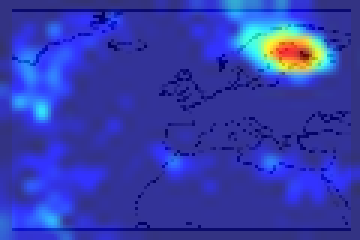
\includegraphics[width=5cm]{paper3_2.png}\\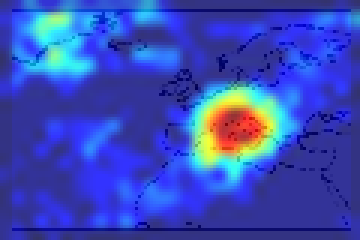
\includegraphics[width=5cm]{paper3_1.png}}\caption{Example of the resulting Class Activation Maps for an ERA-Interim CNN trained using the observed precipitation at Helsinki-Vantaa airport, EFHK, (left) and Rome Fiumicino airport, LIRF, (right). Coastlines have been overlaid as a reference for readers.}\label{paper3}
\end{figure}


\subsection{Publication: Automating weather forecasts based on convolutional networks}

This work was accepted for the "Deep Structured Prediction" workshop celebrated as part of the 2017 ICML conference in Sydney. The work was presented in July 2017 at the workshop and I received positive feedback on the techniques and a few people asked about the nature and availability of the dataset.

\blankpages{10}

%----------------------------------------------------------------------------------------

\section{Convolutional encoder-decoders for image to image regression}

\subsection{Introduction}
The work presented at the 2017 ICML conference led and motivated us to continue researching the field and applications of Convolutional Neural Networks (CNN). Being aware of the demonstrated capacity that CNNs have to extract the spatial structure from input images, we decided to explore the possibilities that these techniques had in the field of meteorology.

For this new research work we focused on studying NWP parameterisations. There are physical processes in the atmosphere that cannot be represented by NWP regardless of its resolution. For these physical processes that cannot be directly resolved, NWP uses approximate models, which are known as parameterisations.

To perform the experiments in this work, we use the ERA-Interim global climate reanalysis dataset produced by the European Centre for Medium-Range Weather Forecasts (ECMWF). ERA-Interim makes available a large number of parameters, from which we choose geopotential height and total precipitation. We crop an extended area over Europe and extracted the selected parameters over the 1980-2016 period with a temporal resolution of 6 hours, resulting in dataset with more than 50,000 samples. 


\subsection{Research contribution}

Autoencoders \citep{hinton2006reducing} are generic neural networks that recreate the input by performing a dimensionality reduction and subsequent expansion of the input space. This technique allows learning compressed representations of the data in an unsupervised manner. Convolutional autoencoders combine CNNs with autoencoders to efficiently learn compressed representations of images. A latter evolution of convolutional autoencoders demonstrates that similar networks offer an efficient way of performing image segmentation by training the model with samples of segmented images. Figure \ref{paper4} contains a representation of the transformations performed by an encoder-decoder network to the geopotential field transforming it into a precipitation field for the same region.

We consider three different state-of-the-art convolutional encoder-decoder networks in the field of image segmentation: VGG-16 \citep{long2015fully}, Segnet \citep{badrinarayanan2017segnet} and U-net \citep{ronneberger2015u}. These networks are modified to perform image regression tasks instead of segmentation by changing the loss function to MAE and tested with the task of predicting precipitation.

This work demonstrates that convolutional encoder-decoder neural networks can be used, as an alternative to parameterisations, to learn complex atmospheric processes using basic NWP fields as input. As far as we know, this is the first attempt to provide an end-to-end automated learning approach to derive new parameterisations from basic NWP fields using deep convolutional encoder-decoder networks. This work also demonstrates how popular deep learning networks in the field of image segmentation can be adapted to interpret and derive new weather parameters.

\begin{figure}[h]
 \centerline{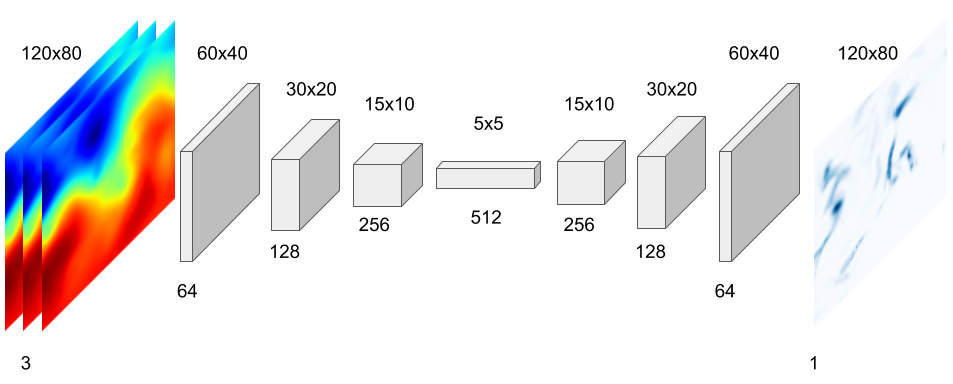
\includegraphics[width=10cm]{paper4.png}}\caption{Representation of the transformations performed by the encoder-decoder network to the geopotential height field and its transformation into a field representing the total precipitation field for the same region.}\label{paper4}
\end{figure}

\subsection{Publication: Learning parameterisations with encoder-decoder convolutional neural networks}

This work has been submitted to the "Monthly Weather Review", which is a peer-reviewed scientific journal published by the American Meteorological Society. It covers research related to analysis and prediction of observed and modeled circulations of the atmosphere, including technique development, data assimilation, model validation, and relevant case studies.

\blankpages{10} 
% Chapter 3

\chapter{Conclusions and future work} % Main chapter title

\label{Chapter3}

This doctoral thesis has been focused on the study of the methodologies and applications of machine learning within the context of weather forecasting. Weather forecasting produces large amounts of data from both observations and numerical simulations. The interpretation of the information contained in these data sets presents interesting challenges in terms of the volume and its high dimensionality. The idea behind our work has been to explore the application of models that can learn to interpret and extract patterns out of these data. In particular, we have explored methodologies that use observed data to enhance the output of numerical simulated weather, and methods for deriving precipitation from basic weather fields. 

\medskip

The first part of this doctoral thesis addresses the application of regression methods using circular variables. Most of the machine learning methodologies available for performing regression are designed to work with linear variables. Circular variables cannot be naturally represented by these algorithms and, in most cases, they are treated as linear variables, which often leads to unsatisfactory results. The first approach that we explored was the idea of using "cyclic kernels" to perform a non-parametric regression of the wind speed. This method allows selecting observed data points around an specific directional component to perform a regression that improves wind speed forecasted by NWP. The second idea that we explored was a method for incorporating circular variables in regression trees. This method builds upon the already existing concept of circular trees proposing a new way of training the trees to improve their accuracy and computational performance.

\medskip

For our third contribution, we changed subject to explore the application of convolutional neural networks into a rain classification or detection problem. Using NWP data as input, treated as an image, we applied convolutional networks to interpret the spatial information contained in these fields and predict the existence of precipitation using observed data for specific collections. This work demonstrates that neural networks can be used to interpret the spatial structure and find correlations with other atmospheric processes, such as precipitation.  

\medskip

Our fourth and last contribution continues exploring the application of convolutional neural networks but with a more challenging task, predicting entire weather fields from  others. In this case, we explored the use of encoder-decoder networks to forecast precipitation using atmospherical pressure fields at several heights. This work demonstrates how convolutional encoder-decoder networks, originally designed to perform segmentation tasks, can be modified to solve difficult problems in the field of weather forecasting, such as learning the physics that relates complex atmospherical processes.

\bigskip
\bigskip
\bigskip

The main contributions in this doctoral thesis can be summarised as follows:

\begin{itemize}
  \item Non-parametric regression can significantly improve NWP fields by eliminating biases.
  \item Cyclic kernels enable non-parametric regression accounting for non resolved topographic effects.
  \item Circular regression trees with contiguous partitions significantly improve the accuracy of regression for circular variables compared to non-contiguous ones.
  \item Our proposed implementation of circular regression trees provides a significant improvement in computational performance and accuracy over the previous version.
  \item Convolutional neural networks can extract the underlying spatial and temporal structure from basic NWP fields.
  \item We deviced a methodology to introspect the weights of convolutional neural networks and determine the regions that are activated for each input.
  \item Convolutional encoder-decoder networks have the capacity to learn the relationships between atmospheric variables. 
  \item This method can be used as an alternative to NWP parameterisations, being U-net the one that offers the best accuracy from all the compared networks.
\end{itemize}

\medskip

This doctoral work was set up and conceived as an exploratory work on the application of machine learning in the field of weather forecasting. In this context, one of the main challenges has been understanding and communicating concepts across both domains and communities. The machine learning community has grown out of the more generic computer science and statistics fields. The weather forecasting community, in spite of having strong ties to the numerical simulation and high performance aspects of computer science, it has been mainly driven along the physics field. For example, some concepts, such as stochastic modeling methods, have been developed in concurrently following different paths, which has resulted in the development of specific terminology to refer to often similar concepts.

\medskip

This challenge has become patent when presenting our ideas to journals belonging to both fields. Although NWP data sets provide an excellent resource for experimenting with generic machine learning algorithms, they require an understanding about the structure and significance of the different variables they represent. Communicating our ideas and contributions to the machine learning community, using a methodological approach, became difficult for the amount of context and domain-specific knowledge required to present our work.

\medskip

The experience has also been similar in the other direction, when presenting our work to weather forecasting audiences. Introducing new machine learning approaches and methodologies to the weather forecasting community has required us to dedicate an special effort in communicating and translating machine learning concepts in the domain-specific language. 

\medskip

Personally, the experience of working in this doctorate during 6 years, has led me to the appreciation of the amount of work required to make contributions in science and a much better understanding of the process. Although my level of understanding about the different machine learning methodologies and techniques has significantly improved through these years, the number of questions and unknowns in my head has only increased. Each of the papers that we published concludes presenting new interesting questions and challenges waiting to be explored.

\medskip

The outcomes of the research we have carried out, have also opened a window for optimism. Realising about the new perspective that machine learning brings to weather forecasting problems and the potential to improve our understanding about the atmosphere has been an encouraging experience. I personally hope to continue learning from and contributing to the development of new links between the machine learning and meteorological communities.
%\include{Chapters/Chapter4} 

%----------------------------------------------------------------------------------------
%	THESIS CONTENT - APPENDICES
%----------------------------------------------------------------------------------------

\appendix % Cue to tell LaTeX that the following "chapters" are Appendices

% Include the appendices of the thesis as separate files from the Appendices folder
% Uncomment the lines as you write the Appendices

% Appendix A

\chapter{A Method for Wind Speed Forecasting in Airports Based on Nonparametric Regression} 
%\afterpage{\null\newpage}\afterpage{\null\newpage}\afterpage{\null\newpage}\afterpage{\null\newpage}\afterpage{\null\newpage}\afterpage{\null\newpage}\afterpage{\null\newpage}\afterpage{\null\newpage}\afterpage{\null\newpage}\afterpage{\null\newpage}

\label{AppendixA} % For referencing this appendix elsewhere, use \ref{AppendixA}


% Appendix B

\chapter{A system for airport weather forecasting based on circular regression trees}

\label{AppendixB} % For referencing this appendix elsewhere, use \ref{AppendixA}
% Appendix C

\chapter{Automating weather forecasts based on convolutional networks}

\label{AppendixC}
% Appendix D

\chapter{Learning parameterisations with encoder-decoder convolutional neural networks}

\label{AppendixD}

%----------------------------------------------------------------------------------------
%	BIBLIOGRAPHY
%----------------------------------------------------------------------------------------

\printbibliography[heading=bibintoc]

%----------------------------------------------------------------------------------------

\end{document}  
